\documentclass[12pt]{report}

% Include all packages from file.
\usepackage[UKenglish]{babel}

\usepackage{setspace}  % LINE SPACING
\usepackage{tikz}
\usepackage{titlepic}
\usepackage{graphicx}
\usepackage{newtxtext,newtxmath}
\usepackage[utf8]{inputenc}
\usepackage[a4paper,left=24.5mm, right=24.5mm, top=24.5mm, bottom=24.5mm]{geometry} %Paper margins
\usepackage{titlesec}
\usepackage{enumitem} % Custom enumerations
\usepackage[titles]{tocloft}

\usepackage{acronym}

\usepackage{hyperref} % Links

% Referencing
\usepackage{natbib} % Harvard referencing
% \usepackage[comma,colon]{natbib}
\citestyle{aysep={,}}
\bibliographystyle{agsm}

% Tables
\usepackage{longtable}
\usepackage{multirow}
\usepackage{xstring}
\usepackage{geometry}
\usepackage{array}


% Fonts size
\usepackage[font={small,it}]{caption}

% Date
\usepackage[useregional]{datetime2}

\usetikzlibrary{calc}
\newcommand\HRule{\rule{\textwidth}{1pt}}
\newcommand{\hsp}{\hspace{10pt}}
\titlespacing*{\chapter}{0pt}{20pt}{20pt} % CHAPTER SPACING
\titleformat{\chapter}[hang]{\Huge\bfseries}{Chapter \thechapter\hsp:\hsp }{0pt}{\Huge\bfseries}
\titleformat{\chapter}[display]{\fontsize{20pt}{0pt}\bfseries}{}{2pt}{}
\setlength{\parindent}{10ex}


% % Setting TOC and Section number depth
% \setcounter{tocdepth}{4}
\setcounter{secnumdepth}{4}
% % line spacing in TOC
\setlength{\cftbeforechapskip}{3pt} 

\onehalfspacing

\usepackage{chngcntr}

% \usepackage[nottoc,numbib]{tocbibind}
\counterwithout{figure}{chapter}
\counterwithout{table}{chapter}

\usepackage[font={small,it}]{caption}
\selectlanguage{UKenglish}

\usepackage{floatrow}

% Header and footer
\usepackage{fancyhdr}
\usepackage{etoolbox}

\usepackage[titletoc]{appendix}
\usepackage{changepage}


% TITLE FORMATS
% CHAPTER SPACING & FONT
\titleformat{\chapter}[hang]{\fontsize{16pt}{0pt}\bfseries}{\thechapter}{1em}{} 
% \titlespacing*{\chapter}{0pt}{20pt}{10pt} 

% SECTION FONT
\titleformat{\section}[hang]{\fontsize{14pt}{0}\bfseries}{\thesection}{1em}{}
% \titlespacing*{\section}{0pt}{20pt}{10pt} 

% SUBSECTION FONT AND SIZE
\titleformat{\subsection}[hang]{\fontsize{12pt}{0}\bfseries}{\thesubsection}{1em}{}
% \titlespacing*{\subsection}{0pt}{15pt}{10pt} 

\titleformat{\subsubsection}[hang]{\fontsize{12pt}{0}\itshape}{\thesubsubsection}{1em}{}
% \titlespacing*{\subsubsection}{0pt}{15pt}{10pt} 

\usepackage{chngcntr}
\counterwithin{table}{chapter}
\counterwithin{figure}{chapter}

\usepackage{makecell}
\usepackage{xargs}
% \usepackage{paralist}

\usepackage{caption}
\usepackage{subcaption}

% \usepackage{acmart}
\newcommand*{\zerospacingchapter}{%
  % CHAPTER SPACING & FONT
\titleformat{\chapter}[hang]{\fontsize{16pt}{0pt}\bfseries}{\thechapter}{1em}{} 
\titlespacing*{\chapter}{0pt}{-10pt}{10pt} 
}

\renewcommand{\contentsname}{Table of Contents}
\renewcommand{\baselinestretch}{1.5}

% HEADER AND FOOTER--------------------------
\patchcmd{\chapter}{\thispagestyle{plain}}{\thispagestyle{fancy}}{}{}
\pagestyle{fancy}
\fancyhf{}
\lhead{\fontsize{10}{12}\leavevmode\selectfont\color{gray}{Lazy-Koala: A Lazy Approach for Root Cause Analysis in Distributed Systems}}
\rfoot{\fontsize{10}{12}\leavevmode\selectfont\color{gray}{\thepage}}
\lfoot{\fontsize{10}{12}\leavevmode\selectfont\color{gray}{Isala Piyarisi | 2018421}}
\renewcommand{\headrulewidth}{0pt}
% END HEADER AND FOOTER--------------------------


% Document begins here
\begin{document}

% TITLE PAGE---------------------------------------------------
\begin{titlepage}

\begin{tikzpicture}[remember picture, overlay]
  \draw[line width = 1pt] ($(current page.north west) + (1cm,-1cm)$) rectangle ($(current page.south east) + (-1cm,1cm)$);
\end{tikzpicture}

\begin{center}

% Upper part of the page
% \text{\large Informatics Institute of Technology}\\[0.1cm]
% \text{\large In Collaboration With}\\[0.5cm]
% \text{\large University of Westminster, UK}\\[2.5cm]

% Title

\includegraphics[width=5.0cm]{assets/IIT-Logo.png}\\[0.7cm]
{ \Huge Anomaly Detection \& Root Cause Analysis\\
In Distributed Systems }\\[0.7cm]
% \begin{minipage}{0.45\textwidth}
\text{\LARGE Project Proposal}\\[0.5cm]

% Authors
% \text{\large A dissertation by}\\[0.1cm]
\text{\large Isala Piyarisi}\\[0.1cm]
\text{\large w1742118 / 2018421}\\[3.2cm]

% Supervisor
\text{\large \textbf{Supervisor}: Guhanathan Poravi}\\[0.1cm]
\text{\large \textbf{Date}: $3^{rd} $ November 2021}\\[0.1cm]
\text{\large \textbf{Department}: Computer Science}\\[0.1cm]
\text{\large \textbf{Keywords}: Cloud Computing, AIOps, Monitoring, Disaster Recovery}\\[5cm]


\large{This project proposal is submitted in partial fulfilment of the requirements for the
BSc(Hons) Computer Science degree at the \\
University of Westminster.
} \\[0.5cm]


\end{center}

\end{titlepage} 

% Page Numbering---------------------------------------------
\pagenumbering{roman}

\chapter*{Abstract}

Cloud computing has shown considerable growth in the past few years, due to its scalability and ease of use. With this change, a new programming paradigm called cloud-native was born. Cloud-native applications are often developed as a set of stand-alone microservices yet could depend on each other to provide a unified experience. Even though microservices introduce a lot of benefits when it comes to flexibility and scalability it could be a nightmare to operate in production. Specifically, when operating a large system with hundreds of microservices talking to each other, the smallest problem could result in failures all around the system.

% Cloud computing is a steady rise for the past few years due to its scalability and ease of use. With this change, a new programming paradigm called cloud-native was born. Cloud-native applications are often developed as a set of stand-alone microservices yet, it could depend on each other to provide a unified experience. 

% This helps different teams to work on different services which increases the development velocity. This works well for medium to large companies but over time this mesh of services could become very complicated to a point where it's very difficult for a single person to understand the entire system. When the system consists of thousands of individual services talking and depending on each other, the network layer of that system becomes chaotic. A failure in a single point could create a ripple effect across the entire system. When something like that happens it could take a considerable amount of time to zero in on the exact point of the failure.

The focus of this project are in two-folds. First, the authors introduce a robust Kubernetes native toolkit that helps both researchers and developers collect and process service telemetry data with zero instrumentation. Secondly, the authors proposed a novel way of detecting anomalies by encoding raw metric data into an image-like structure and using a convolutional autoencoder to learn the general data distribution for each service and detecting outliers. Finally, a weighted graph was used along with anomaly scores calculated prior to finding out possible root cause for any system anomaly.

Initial test results show that the telemetry extraction components are both resilient and lightweight even under the sustained load, while the anomaly prediction algorithm seems to converge on target learning goals.
\newline
\newline
\textbf{Keywords}:
AIOps, Monitoring, Disaster Recovery, eBPF, Kubernetes
\newline
\textbf{Subject Descriptors}:
• Computing methodologies $\rightarrow$ Machine learning $\rightarrow$ Learning paradigms $\rightarrow$ Unsupervised learning $\rightarrow$ Anomaly detection • Computer systems organization $\rightarrow$ Architectures $\rightarrow$ Distributed architectures $\rightarrow$ Cloud computing
\addcontentsline{toc}{chapter}{Abstract}

% Table of Contents---------------------------------------------------
\tableofcontents
% List of Figures---------------------------------------------------
% \cleardoublepage
{\let\clearpage\relax
\listoffigures
}
\addcontentsline{toc}{chapter}{\listfigurename}
% List of Tables---------------------------------------------------
{\let\clearpage\relax 
\listoftables
}
\addcontentsline{toc}{chapter}{\listtablename}

% \cleardoublepage
\phantomsection
% Include acronyms
\addcontentsline{toc}{chapter}{List of Acronyms}
% {\let\clearpage\relax 
\chapter*{List of Acronyms}

\begin{acronym}
% \acro{iaas}[IaaS]{Infrastructure as a Service}
\acro{sres}[SRE]{Site Reliability Engineer}
\acro{sli}[SLI]{Service Level Indicator}
\acro{sre}[SRE]{Site Reliability Engineering}
\acro{apm}[APM]{Application Performance Monitoring}
\acro{mttr}[MTTR]{Mean Time To Recovery}
% \acro{gan}[GAN]{Generative adversarial networks}
% \acro{hhmm}[HHMM]{Hierarchical hidden Markov model}
% \acro{fsl}[FSL]{Few-shot Learning}
% \acro{sdlc}[SDLC]{Software Development Life Cycle}
% \acro{ooad}[OOAD]{Object-oriented analysis and design}
\acro{ebpf}[eBPF]{Extended Berkeley Packet Filter}
% \acro{sla}[SLA]{Service-Level Agreement}
% \acro{saas}[SaaS]{Software as a service}
% \acro{vm}[VM]{Virtual Machine}
% \acro{cncf}[CNCF]{Cloud Native Computing Foundation}

\acro{aiops}[AIOps]{Artificial Intelligence for IT operations}
% \acro{sre}[SRE]{Site Reliability Engineering}
\acro{gazer}[Gazer]{Telemetry extraction agent}
\acro{sherlock}[Sherlock]{AI-engine}
\acro{lazy-koala-operator}[Operator]{Lazy Koala Resource Manager}
\end{acronym}
% }
\zerospacingchapter
\chapter{Introduction}
\pagenumbering{arabic}
\section{Chapter Overview}

The following chapter presents the evaluation process of this project and its findings. It starts by explaining the evaluation methodology and criteria for the project will be evaluated. The author then discusses their thoughts on the final product of this research. Then the thought process behind the selection evaluator will be explained. Finally, the chapter will conclude with feedback provided by the evaluators along with potential limitations in the evaluation.
\section{Problem Domain}

\subsection{Cloud Computing}
With an emergence of Infrastructure as a Services (IaaS) like Amazon Web Services (AWS) and Google Cloud Platform (GCP) there is a big surge in organizations trying to outsource their computing needs to third parties \citep{rimol_2021}. This is mainly due to the elasticity given by all the cloud providers. Users can easily scale up and down their infrastructures within minutes without making any commitment. All the major providers bill users on "what you use is what you pay model". Since the cloud provider manages all the underlying infrastructure, users doesn't have to worry about problems like hardware failures. In contrast in a self-hosted setting if the user wanted one extra GB of memory than what's available it requires a lot of effort and it cost a lot to full fill that requirement.

\subsection{Cloud-Native Applications}
During the 90s and early 2000s, all the applications were made as a big monolith from a single code base \citep{LessonsF52:online}. Most of them were shipped as a single binary. Since those days applications were fairly simple this worked very well with little to no downsides. When the 2010s came around there were a lot of specialized frameworks and programming languages and marketing teams wanted a lot of new futures quickly developed still maintaining reliability \citep{di2018migrating,Microser52:online}. But if the code base of the application was stored in a single repository, developers have to go through a long process to review and test if the changes won't break the current systems. Developers are also limited by the frameworks and programming languages that were chosen for the project at the start.

To tackle these problems a new way to develop applications was introduced, it's called "Microservices". The idea behind this concept is to break all the functionalities of big monolithic applications into small individually scalable services and give ownership of each service to small teams of people who work separately. With this flow developers are free to use whatever tool they like to develop each service. Because these services are developed parallelly by different teams this increases the development velocity by order of magnitude \citep{Understa56:online}.

As these services are relatively small and tailor-made to run on cloud environments it's easier to take something that's running on the developer's local machine to the production cluster in a matter of minutes. This is mainly thanks to modern cloud-native tools like CI/CD pipelines which automatically build and test the code for them, which can save a lot of time spent just doing repetitive tasks which are prone to human errors \citep{Whataret68:online}.

\subsection{Monitoring Cloud-Native Applications} \label{monitoring-bg}
Even though cloud-native applications have a lot to offer when it comes to developer velocity and productivity, It has its fair share of issues. Most of these problems are linked to the sheer complexity of these systems and not having a proper way to monitor them \citep{5WaysYou35:online}. All 3 major cloud providers provide a way to monitor these applications efficiently and there are some great open-source projects do this well, But to take full advantage of those systems, developers have to adapt their services to export all the vitals in a way the monitoring system understand. This works for the most part and this is what all the big companies are doing, even if it takes more developer time to in the end it's very crucial when it comes to disaster recovery.

But there is still a slight problem with this approach. Once the system starts to scale up to hundreds of services, the number vitals that has to be monitored goes to thousands and will require a lot of additional \acp{sres} and will have drop to lot of non-crucial service vitals and derive abstract \acp{sli} to make it \textbf{humanly} possible to understand what's going on.\\

\section{Problem Definition}

One of the leading problems in monitoring microservices is the sheer number of data that they generate. It's humanly impossible to monitor the metrics of all the services and it's hard for a single person to understand the entire system. By\acp{sres} using abstracted metrics called \acp{sli} which measures the quality of the service at a higher level can overcome this. Although \acp{sli} can alert when there is an issue in the system, it is difficult to understand where the actual problem is from this point on. To understand the root cause of the problem, \acp{sres} need to dig into \acp{apm} of all the services and go through each and every log of the troubling services.

When the system consists of hundreds or thousands of services that are interdependent; It is really hard to find where the actual issue is coming from and it may require the attention from all the service owners of the failing services to go through the logs and \acp{apm} to identify the actual root cause of the failure. This could greatly increase the \ac{mttr} and waste a lot of developer time by browsing logs.

\subsection{Problem Statement}

Modern distributed systems are becoming large and complex to the point where, when a failure occurs, it requires collaboration with a large number of people to find the actual root cause. Implementing a \textbf{framework} to make it easier to integrate machine learning models to detect anomalies in real-time could deflate \ac{mttr}.
\section{Existing Work}

\subsection{Anomaly detection}

\begin{longtable}{| p{20mm} | p{43mm} | p{43mm} | p{43mm} |}
\hline
  \textbf{Citation} &
  \textbf{Technology summary} &
  \textbf{Improvements} &
  \textbf{Limitations} \\ \hline


  \cite{du2018anomaly} &
  Tested most of common machine learning methods to detect anomalies and benchmarked them &
  \vspace{-8mm}
  \begin{itemize}[leftmargin=*,noitemsep,nolistsep] 
    \item Used \acp{sli} to monitored data
    \item A lot of good metrics (input data)
    \item Performance monitoring of services and containers
  \vspace{-7mm}
  \end{itemize} &
  \vspace{-8mm}
  \begin{itemize}[leftmargin=*,noitemsep,nolistsep] 
    \item Only be able to identify predetermined issues
    \item Require a sidecar that includes a lot of overheads
    \item Won't work with event-driven architectures (this is where most of the new systems are headed)
    \item Uses Supervised learning and it is nearly impossible to find real-world data with labels
  \vspace{-7mm}
  \end{itemize} \\ \hline


  \cite{kumarage2018anomaly} &
  The authors here propose a semi-supervised technique using a Variational Autoencoder to predict future time steps and calculate the difference between predicted and actual to detect anomalies. &
  \vspace{-8mm}
  \begin{itemize}[leftmargin=*,noitemsep,nolistsep] 
    \item Due to the difficulty of finding labelled research data, they settled on using a semi-supervised technique.
    \item Randomized decision trees used were used to select the most suitable characteristics for each component.
  \vspace{-7mm}
  \end{itemize} &
  \vspace{-8mm}
  \begin{itemize}[leftmargin=*,noitemsep,nolistsep] 
    \item The model will not be effortlessly transformable for other systems
    \item If more new key features were added to the system it will require a total retraining
  \vspace{-7mm}
  \end{itemize} \\ \hline


  \cite{kumarage2019generative} &
  Uses a bidirectional GAN to predict future timesteps and uses MSE between prediction and real to determine the anomalies &
  Experimented using a GAN to detect anomalies rather than using conventional autoencoders &
  \vspace{-8mm}
  \begin{itemize}[leftmargin=*,noitemsep,nolistsep] 
    \item Accuracy is around 60\%, which is unimpressive for use in production with mission-critical systems.
    \item As this is a GAN-based system, it may take numerous resources to run with production systems.
  \vspace{-7mm}
  \end{itemize} \\ \hline


  \caption{Comparison of anomaly detection methods in distributed systems (self-composed)}
\end{longtable}

\subsection{Root cause identification}

\begin{longtable}{| p{20mm} | p{40mm} | p{43mm} | p{46mm} |}
\hline
  \textbf{Citation} &
  \textbf{Technology summary} &
  \textbf{Improvements} &
  \textbf{Limitations} \\ \hline


  \cite{gonzalez2017root} &
  Detect failures in networks, using machine learning to generate knowledge graphs on historical data &
  \vspace{-8mm}
  \begin{itemize}[leftmargin=*,noitemsep,nolistsep] 
    \item Predictable system
    \item Automatic identification of dependencies between system events
    % \item independent of Domain experts
    \item Generalized to various systems
  \vspace{-7mm}
  \end{itemize} &
  \vspace{-8mm}
  \begin{itemize}[leftmargin=*,noitemsep,nolistsep] 
    \item Limited to network issues
    \item \acp{sres} must manually identify the issues, although the knowledge graph helped visualisation.
  \vspace{-7mm}
  \end{itemize} \\ \hline


  \cite{chigurupati2017root} &
  Proposed a way to detect hardware failures in servers using a probabilistic graphical model that concisely describes the relationship between many random variables and their conditional independence &
  \vspace{-8mm}
  \begin{itemize}[leftmargin=*,noitemsep,nolistsep] 
    \item Find hidden meaning in values that seems random
    \item Used a probabilistic approach to understand the relationship between inputs and outputs more clearly
    \item Gives all the possible root causes for a given problem
  \vspace{-7mm}
  \end{itemize} &
  \vspace{-8mm}
  \begin{itemize}[leftmargin=*,noitemsep,nolistsep] 
    \item Limited to hardware issues
    \item Require support from domain experts
    \item Can't account for unforeseen errors
  \vspace{-7mm}
  \end{itemize} \\ \hline


  \cite{wu2020microrca} &
  Find Performance bottlenecks in distributed systems using an attribute graph to find anomaly propagation across services and machines &
  \vspace{-8mm}
  \begin{itemize}[leftmargin=*,noitemsep,nolistsep] 
    \item Created a custom Fault Injection module
    \item Uses an attribute graph to localise to faulty service
    \item Application-agnostic by using a service mesh
    \item Rely on the service mesh to determine network topology
    \item Uses unsupervised learning
  \vspace{-7mm}
  \end{itemize} &
  \vspace{-8mm}
  \begin{itemize}[leftmargin=*,noitemsep,nolistsep] 
    \item Only able to identify 3 types of issues
    \item Checks only for performance anomalies
    \item Use the slow response time of a microservice as the definition of an anomaly
    \item Service meshes add a lot of overhead to systems
    \item Required direct connection between services
  \vspace{-7mm}
  \end{itemize} \\ \hline


  \cite{samir2019dla} &
  This detects and locates the anomalous behavior of microservices based on the observed response time using a HHMM &
  \vspace{-8mm}
  \begin{itemize}[leftmargin=*,noitemsep,nolistsep] 
    \item Custom HHMM model
    \item Self-healing mechanism
    \item Focus on performance detection and identification at the container, node, and service level
  \vspace{-7mm}
  \end{itemize} &
  \vspace{-8mm}
  \begin{itemize}[leftmargin=*,noitemsep,nolistsep] 
    \item The input data set scale is limited
    \item Require a sidecar
    \item Needs to predetermined thresholds
  \vspace{-7mm}
  \end{itemize} \\ \hline


  \caption{Comparison of root cause identification methods in distributed systems (self-composed)}
\end{longtable}

\subsection{Commercial products}

\begin{longtable}{| p{40mm} | p{55mm} | p{55mm} |}
\hline
  \textbf{Name} &
  \textbf{Futures} &
  \textbf{Limitations} \\ \hline


  Applied Intelligence by New Relic &
  \vspace{-8mm}
  \begin{itemize}[leftmargin=*,noitemsep,nolistsep] 
    \item Metric forecasting.
    \item Anomaly detection.
    \item Alert grouping to reduce noise.
  \vspace{-7mm}
  \end{itemize} &
  \vspace{-8mm}
  \begin{itemize}[leftmargin=*,noitemsep,nolistsep] 
    \item Lack of explanation for certain classifications.
    \item All the telemetry data need to be sent to a third party.
  \vspace{-7mm}
  \end{itemize} \\ \hline


  Watchdog by Datadog &
  \vspace{-8mm}
  \begin{itemize}[leftmargin=*,noitemsep,nolistsep] 
    \item Monitor the metric data of the entire system from the background.
    \item Monitor the log data.
    \item Highlight relevant components affected by an issue.
  \vspace{-7mm}
  \end{itemize} &
  \vspace{-8mm}
  \begin{itemize}[leftmargin=*,noitemsep,nolistsep] 
    \item Announced in 2018 but is still in private beta.
    \item Require code changes and tight integration with the datadog platform.
    \item Available demos about the system seem to be designed for demonstration purposes.
  \vspace{-7mm}
  \end{itemize} \\ \hline


  \caption{Comparison of commercial products for root cause analysis (self-composed)}
\end{longtable}
\section{The Novelty of the Research}

\subsection{Problem Novelty}

After a literature survey, the author concluded that finding the root cause of any failure within a distributed system is a challenging issue. This is mainly due to the fact that this problem cannot be assigned to a fixed set of inputs and outputs, which is a basic requirement for almost all types of neural network that are readily available. 

% Furthermore, almost all the researchers working on this problem domain have built their own solution for simulating a distributed system, since there isn't any open dataset on service monitoring. This could be mainly due to the fact that these datasets could contain sensitive information. 

Most of the currently established research was done towards creating statistical models like clustering and linear regression. Although these algorithms perform outstandingly in small-scale systems, they can struggle to adapt in the large-scale, noisy monitoring data found in medium-to large-sized systems. Another problem that was recognised was that none of these articles adequately addressed the issue of constant changes in services. Most published research considers target services static, but, in fact, these services can change constantly within a day \citep{GoingtoM51:online}. Finally, non of the published work has addressed the issue of scaling the anomaly detection system relative to the target distributed system which is a crucial factor for production use.

\subsection{Solution Novelty}


The focus of this project is to create an adaptable and scalable series of components that ranges from instrumentation to root cause analysis, which can be well integrated into an existing system or can be extended to fit to newer use cases. To achieve this the author is utilizing a fairly new technique called \ac{ebpf} for instrumentation, which is a Linux kernel API that can be used to track kernel events such as TCP socket changes to identify and understand the network layer of each application running on the system. Finally, for anomaly detection, a convolutional autoencoder with a novel data encoding method was used to keep the system as lightweight as possible, while still having acceptable accuracies for classifications. Combining that with a directed graph generated from collected network activity data can be used to highlight to blast radius of an anomaly along with possible causes.

\section{Research Question}


\begin{enumerate}[leftmargin=*,label=\textbf{RQ\arabic*:}]

\item How can a machine learning model improve \ac{mttr} in a distributed system?

\item What is the most efficient way to present raw data monitoring to machine learning model?

\item What will be the most ideal machine learning model to uncover anomalies in a microservice?

\item What are the methods that can be used to evaluate a root cause prediction system?

\end{enumerate}



\section{Research Motivation}

Modern distributed systems generate tons of useful and useless telemetry data. As the demand and size of the system increases, these telemetry data become more nosier and more complex \citep{Untangli35:online}. It makes difficult for humans to understand all these data, especially if they do not have long-standing experience with the system. On the other hand, deep learning models thrive when they have no end of data to learn from. As these models can be trained in computer-simulated environments, they can learn concepts that humans need years to grasp, within days \citep{OpenAI_dota, silver2017mastering}. Finally, unlike humans a deep learning model can monitor a service 24x7 without taking any breaks which will not only prevent outages even before they happen, It could be reduced \ac{mttr} because the issue can be detected way earlier than any human could do. 
\section{Research Challenge \& Potential}

% Even though this project seems very straightforward and easy to implement from a high level, it becomes problematic when it comes to reaching targets the author has set for himself. For an example, interpretability was one of the most requested features from the industry experts and a must-have trait for mission-critical systems \citep{ribeiro2016should}. But it was left out of the project scope due to its complexity especially when it comes to an undergraduate level project. Other than that following are a few of the more difficult challenges the author is expected to face while conducting the research.

\subsection{Research Challenge}

\begin{itemize}[leftmargin=*] 
    \item \textbf{Highly seasonal and noisy patterns} - Monitoring metrics on microservices in production tend to have very unpredictable patterns depending on the traffic that has been sent to the service. The amount of traffic sent will depend on several external factors that are hard to determine. Modeling both temporal dependencies and static interdependencies found in telemetry data of services into a single graph will be very difficult and require a lot of fine-tuning and data engineering skills.
    \item \textbf{Overhead} - Modern deep learning models can solve any problem if we could give them an unlimited amount of data and processing power. Although in this case, the models need to optimize for efficiency over accuracy since having a monitoring system that consumes a lot more resources than the actual target system isn't effective.
    \item \textbf{Fit into Kubernetes eco-system} - Kubernetes has become the de facto standard for managing distributed systems \citep{WhatisCo78:online}. So the author is planning to create a Kubernetes extension that will bridge the connection between monitored service and monitoring model. But Kubernetes itself has a very steep learning curve, even the original developers themselves have admitted that Kubernetes is too hard and complex for beginners \citep{Googlead4:online}.
    \item \textbf{Extraction of Telemetry} - Even though it's considered the best practice to implement telemetry exporting methods in the development phase of any application, developers often skip this part to save time. Sometimes it's required to depend on external applications that are developed by third parties which don't have means of exporting telemetry. Additionally, when building an end-to-end root course indication platform, it is required to take these kinds of scenario into account.
\end{itemize}

\subsection{Research Potential}

The feedback received for this project has been very positive because this is a very common but still unsolved issue in reliability engineering. Since this project was developed as a set of loosely coupled components, some of the experts expressed their interest in using individual components to solve some of the other problems they have been experiencing over time. Finally, this project can be used as an initial point for future research that focusses on specific areas of \ac{aiops} by replacing the individual components of this with their own.
\section{Research Aim}

\textit{The aim of this research is to design, develop and evaluate a low overhead Kubernetes framework to collect, store and process telemetry data using deep learning to help system operators detect anomalies earlier in order to reduce the \ac{mttr} when the system is experiencing an anomaly.}

In this project, the author tries to create a single model that can monitor all the vitals of a given service and output an anomaly score in any given time window. The author hopes to make it general enough so that operators can take the same model and deploy it with other services, and the model will be adopted to the new services using a few-shot learning method \citep{wang2020generalizing}. To make it happen, the author is trying to create a data encoding technique to represent monitoring data in a programming language/framework-independent way. To achieve this goal the author is also hoping to create a lightweight service instrumentation pipeline that can collect and process telemetry data in real-time without requiring any additional work from the user's end.
\section{Research Objectives}

\newcommand\robProblemIdentification{
When selecting the problem the author wanted to pursue, they had three main goals.
\begin{enumerate}[leftmargin=*,noitemsep,nolistsep,label=RO\arabic*:] 
    \item The problem domain should be something they would enjoy working on.
    \item At the end of the research they should give a meaningful impact to the target domain, both in the theoretical and practical aspect.
    \item It should be challenging to achieve, and the results should speak for themselves.
    \vspace{-7mm}
\end{enumerate}
}

\newcommand\robLiteratureReview{
Conduct a Literature review on root cause analysis, 
\begin{enumerate}[leftmargin=*,noitemsep,nolistsep,label=RO\arabic*:] 
    \setcounter{enumi}{3}
    \item To find the current methods that are used for anomaly detection and root cause localization.
    \item Uncover issues with current approaches.
    \item Understand how advancements in other related domains can apply to this domain.
    \vspace{-7mm}
\end{enumerate}
}


\newcommand\robDevelopingEvaluation{
During the literature survey, one of the problems the author identified was that there is no uniform data set when it comes to training or evaluating models to detect anomalies in microservices. Most of the researchers used private datasets to train and test their work.
To address this, the author is developing
\begin{enumerate}[leftmargin=*,noitemsep,nolistsep,label=RO\arabic*:] 
    \setcounter{enumi}{5}
    \item A tool that can easily simulate a distributed system in a cloud-native setting.
    \item A tool that can inject anomalies into the running services.
    \vspace{-7mm}
\end{enumerate}
}

\newcommand\robPublishPlayground{
The author hopes to publish a paper on the above-mentioned tool so that future researchers will have a unified way to train, test, and benchmark their system without having to reinvent the wheel again and again.
}

\newcommand\robDataGathering{
To create a model to detect anomalies, the author will have to
\begin{enumerate}[leftmargin=15mm,noitemsep,nolistsep,label=RO\arabic*:] 
    \setcounter{enumi}{7}
    \item Simulate a distributed system.
    \item Simulate the traffic inside the system.
    \item Collect monitoring data while it's running.
    \vspace{-7mm}
\end{enumerate}
}

\newcommand\robDevelopingEncoding{
Since these microservices will report very different metric values even at idle depending on the architecture of the service. To normalize theses data points from all the services to one format author will,
\begin{enumerate}[leftmargin=15mm,noitemsep,nolistsep,label=RO\arabic*:] 
    \setcounter{enumi}{10}
    \item Evaluate current data encoding methods such as \cite{zhang2019deep}.
    \item Find the best fit and optimise it for this use case.
    \item Test if there is improvement by using that method. 
    \vspace{-7mm}
\end{enumerate}
}


\newcommand\robDevelopingModel{
According to \cite{kumarage2019generative}, autoencoders tend to perform best when it comes to anomaly detection. But during the literature survey it was revealed that convolution autoencoders weren't tested for this usecase. So, the author is hoping to develop a convolution auto-encoder and test how it will perform.
}


\newcommand\robTesting{
The following things will be tested during the testing phase, 
\begin{enumerate}[leftmargin=15mm,noitemsep,nolistsep,label=RO\arabic*:] 
    \setcounter{enumi}{13}
    \item How will the system classify long-term \& short-term fluctuations.
    \item What will be the overhead of the system.
    \item Can the system understand the mapping between core metrics like CPU and Memory usages.
    \item Accuracy of fault detection.
    \item Reliability of the instrumentation system.
\vspace{-7mm}
\end{enumerate}
}

\newcommand\robIntegration{
Having a fancy model does not add anything if it is very hard to use with a real system. So the author is hoping to develop a Kubernetes extension that will map the model with any service given by the user.
}


\begin{longtable}{|p{20mm}|p{90mm}|p{19mm}|p{17mm}|}
\hline
    \textbf{Research Objectives} &
    \textbf{Explanation} &
    \textbf{Learning Outcomes} &
    \textbf{Research Questions} \\ \hline

    Problem identification &
    \robProblemIdentification &
    LO1 &
    RQ1, RQ3 \\ \hline

    Literature review &
    \robLiteratureReview &
    LO3, LO4, LO6 &
    RQ1, RQ2, RQ3, RQ4 \\ \hline

    Developing an evaluation framework &
    \robDevelopingEvaluation &
    LO7 &
    RQ4 \\ \hline

    % Publish a paper on that playground &
    % \robPublishPlayground &
    % LO7 &
    % N/A \\ \hline

    Data gathering and analysis &
    \robDataGathering &
    LO7 &
    RQ2, RQ4 \\ \hline

    Developing the encoding method &
    \robDevelopingEncoding &
    LO2, LO5, LO7 &
    RQ2, RQ3 \\ \hline

    Developing the model &
    \robDevelopingModel &
    LO2, LO5, LO7 &
    RQ4 \\ \hline

    Testing and evaluation &
    \robTesting &
    LO8, LO9 &
    RQ1, RQ3, RQ4 \\ \hline

    Integration &
    \robIntegration &
    LO7 &
    RQ1, RQ3 \\ \hline

\caption{Research Objectives (self-composed)}
\end{longtable}

\section{Research Contribution}


\subsection{Domain Contribution}

With this research, the author first tried to develop a \textbf{cloud-native solution to create a configurable microservices system}, so this research and future research will have a standard environment to develop and evaluate their work. The author built a lightweight and \textbf{low-overhead data collection pipeline} using \ac{ebpf} to collect telemetry of target services without any instrumentation from the user.

\subsection{Knowledge Contribution}

One of the main problems with monitoring microservices systems is that different services can be developed with different programming languages and frameworks, and those can contain different levels of noise\label{need-for-encoding}. Therefore, it is complicated for a single model to detect anomalies in any service since some frameworks tend to use more resources while idle than others. To address this author is trying to come up with an \textbf{encoding method} so the model can be trained to monitor one framework and those learning will still be valid for another framework. With these encoded data, the author is hoping to develop a \textbf{convolutional autoencoder that will use unsupervised learning to spot out anomalies in a given data stream}. This may have better performance while using fewer resources since convolutional layers are typically lightweight and good at pattern recognition \citep{oord2016wavenet}. Finally, the author plans to aggregate these predictions from the models into a pre-generated service graph and weigh them at \textbf{find all possible root causes}.

{\let\clearpage\relax\chapter{Project Scope}}

From the literature survey and talking with industry, experts author found many issues they can address when developing the system, but some of those problems like interpretability on autoencoder \citep{ribeiro2016should} are hard to solve by someone at a level of an undergraduate. As this project is done by one developer in less than one year, it won't be possible to create a fully functional monitoring platform like Datadog or New Relic. The Force of this project is to see if the author can develop a single model that can monitor all kinds of services after transfer learning with few examples. \\

\newpage

\section{In-scope} \label{sec:in-scope}
Following are the main forces of this project
\begin{itemize}[noitemsep,nolistsep] 
    \item Evaluation Framework
    \begin{itemize}[noitemsep,nolistsep] 
        \item Ability to create service mesh out using Kubernetes native resources.
        \item Each service has the ability to simulator predefined error types.
        \item Service mesh can be made up of services written in different programming languages and  frameworks.
        \item Built-in method to run stress tests.
    \end{itemize}
    \item Monitoring System
    \begin{itemize}[noitemsep,nolistsep]
        \item Low overhead data collection pipeline to collect service telemetry.
        \item Reliability system which generate fewer false positives so it won't overwhelm the operators and false negatives will be caught by the main monitoring system.
        \item Optimized models to have fairly small memory footprint and a CPU overhead.
        \item Well generalized model which will be able to deploy with completely new services and it will learn to adapt the new system.
    \end{itemize}
\end{itemize}


% \item Constant changes to services
% \item Highly seasonal and noisy patterns 
% \item few shot learning to convert to a new system
% \item Tunability
% \item Reponsed to seasonal dependencies 
% \end{enumerate}



\section{Out-scope} \label{sec:out-scope}
Follow will not be covered during this project
\begin{itemize}[noitemsep,nolistsep] 
    \item Evaluation Framework
    \begin{itemize}[noitemsep,nolistsep] 
        \item Support for every major language and framework.
        \item Working outside of Kubernetes eco-system.
    \end{itemize}
    \item Monitoring System
    \begin{itemize}[noitemsep,nolistsep] 
        \item Interpretability - Describing a behavior of autoencoder is a difficult task that won't be covered during the project.
        \item System won't be trained against data from a real production system due to the lack of public datasets.
        \item System won't have very high accuracy, as this will be the first line of defense this will try to avoid false positives to prevent adding more noise to alerting systems.
        \item Automatically identify system topology.
        \item This will not be a drop-in replacement for existing monitoring systems, rather this will work with existing monitoring systems to reduce the \ac{mttr}.
    \end{itemize}
\end{itemize}

\section{Prototype Feature Diagram}
\begin{figure}[H]
    \centering
    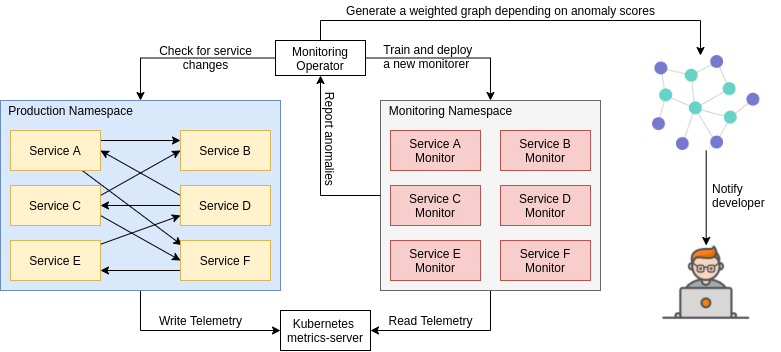
\includegraphics[width=16cm]{assets/High-level-system-diagram.png}
    \caption{Prototype feature diagram (self composed)}
    \label{fig:high-level-diagram}
\end{figure}
\section{Chapter Summary}

The above chapter described the participation of social, legal, ethical and professional issues in this project and how those were mitigated to comply with the BCS code of conduct.
\chapter{Introduction}
\pagenumbering{arabic}
\section{Chapter Overview}

The following chapter presents the evaluation process of this project and its findings. It starts by explaining the evaluation methodology and criteria for the project will be evaluated. The author then discusses their thoughts on the final product of this research. Then the thought process behind the selection evaluator will be explained. Finally, the chapter will conclude with feedback provided by the evaluators along with potential limitations in the evaluation.
\section{Problem Domain}

\subsection{Cloud Computing}
With an emergence of Infrastructure as a Services (IaaS) like Amazon Web Services (AWS) and Google Cloud Platform (GCP) there is a big surge in organizations trying to outsource their computing needs to third parties \citep{rimol_2021}. This is mainly due to the elasticity given by all the cloud providers. Users can easily scale up and down their infrastructures within minutes without making any commitment. All the major providers bill users on "what you use is what you pay model". Since the cloud provider manages all the underlying infrastructure, users doesn't have to worry about problems like hardware failures. In contrast in a self-hosted setting if the user wanted one extra GB of memory than what's available it requires a lot of effort and it cost a lot to full fill that requirement.

\subsection{Cloud-Native Applications}
During the 90s and early 2000s, all the applications were made as a big monolith from a single code base \citep{LessonsF52:online}. Most of them were shipped as a single binary. Since those days applications were fairly simple this worked very well with little to no downsides. When the 2010s came around there were a lot of specialized frameworks and programming languages and marketing teams wanted a lot of new futures quickly developed still maintaining reliability \citep{di2018migrating,Microser52:online}. But if the code base of the application was stored in a single repository, developers have to go through a long process to review and test if the changes won't break the current systems. Developers are also limited by the frameworks and programming languages that were chosen for the project at the start.

To tackle these problems a new way to develop applications was introduced, it's called "Microservices". The idea behind this concept is to break all the functionalities of big monolithic applications into small individually scalable services and give ownership of each service to small teams of people who work separately. With this flow developers are free to use whatever tool they like to develop each service. Because these services are developed parallelly by different teams this increases the development velocity by order of magnitude \citep{Understa56:online}.

As these services are relatively small and tailor-made to run on cloud environments it's easier to take something that's running on the developer's local machine to the production cluster in a matter of minutes. This is mainly thanks to modern cloud-native tools like CI/CD pipelines which automatically build and test the code for them, which can save a lot of time spent just doing repetitive tasks which are prone to human errors \citep{Whataret68:online}.

\subsection{Monitoring Cloud-Native Applications} \label{monitoring-bg}
Even though cloud-native applications have a lot to offer when it comes to developer velocity and productivity, It has its fair share of issues. Most of these problems are linked to the sheer complexity of these systems and not having a proper way to monitor them \citep{5WaysYou35:online}. All 3 major cloud providers provide a way to monitor these applications efficiently and there are some great open-source projects do this well, But to take full advantage of those systems, developers have to adapt their services to export all the vitals in a way the monitoring system understand. This works for the most part and this is what all the big companies are doing, even if it takes more developer time to in the end it's very crucial when it comes to disaster recovery.

But there is still a slight problem with this approach. Once the system starts to scale up to hundreds of services, the number vitals that has to be monitored goes to thousands and will require a lot of additional \acp{sres} and will have drop to lot of non-crucial service vitals and derive abstract \acp{sli} to make it \textbf{humanly} possible to understand what's going on.\\

\section{Problem Definition}

One of the leading problems in monitoring microservices is the sheer number of data that they generate. It's humanly impossible to monitor the metrics of all the services and it's hard for a single person to understand the entire system. By\acp{sres} using abstracted metrics called \acp{sli} which measures the quality of the service at a higher level can overcome this. Although \acp{sli} can alert when there is an issue in the system, it is difficult to understand where the actual problem is from this point on. To understand the root cause of the problem, \acp{sres} need to dig into \acp{apm} of all the services and go through each and every log of the troubling services.

When the system consists of hundreds or thousands of services that are interdependent; It is really hard to find where the actual issue is coming from and it may require the attention from all the service owners of the failing services to go through the logs and \acp{apm} to identify the actual root cause of the failure. This could greatly increase the \ac{mttr} and waste a lot of developer time by browsing logs.

\subsection{Problem Statement}

Modern distributed systems are becoming large and complex to the point where, when a failure occurs, it requires collaboration with a large number of people to find the actual root cause. Implementing a \textbf{framework} to make it easier to integrate machine learning models to detect anomalies in real-time could deflate \ac{mttr}.
\section{Existing Work}

\subsection{Anomaly detection}

\begin{longtable}{| p{20mm} | p{43mm} | p{43mm} | p{43mm} |}
\hline
  \textbf{Citation} &
  \textbf{Technology summary} &
  \textbf{Improvements} &
  \textbf{Limitations} \\ \hline


  \cite{du2018anomaly} &
  Tested most of common machine learning methods to detect anomalies and benchmarked them &
  \vspace{-8mm}
  \begin{itemize}[leftmargin=*,noitemsep,nolistsep] 
    \item Used \acp{sli} to monitored data
    \item A lot of good metrics (input data)
    \item Performance monitoring of services and containers
  \vspace{-7mm}
  \end{itemize} &
  \vspace{-8mm}
  \begin{itemize}[leftmargin=*,noitemsep,nolistsep] 
    \item Only be able to identify predetermined issues
    \item Require a sidecar that includes a lot of overheads
    \item Won't work with event-driven architectures (this is where most of the new systems are headed)
    \item Uses Supervised learning and it is nearly impossible to find real-world data with labels
  \vspace{-7mm}
  \end{itemize} \\ \hline


  \cite{kumarage2018anomaly} &
  The authors here propose a semi-supervised technique using a Variational Autoencoder to predict future time steps and calculate the difference between predicted and actual to detect anomalies. &
  \vspace{-8mm}
  \begin{itemize}[leftmargin=*,noitemsep,nolistsep] 
    \item Due to the difficulty of finding labelled research data, they settled on using a semi-supervised technique.
    \item Randomized decision trees used were used to select the most suitable characteristics for each component.
  \vspace{-7mm}
  \end{itemize} &
  \vspace{-8mm}
  \begin{itemize}[leftmargin=*,noitemsep,nolistsep] 
    \item The model will not be effortlessly transformable for other systems
    \item If more new key features were added to the system it will require a total retraining
  \vspace{-7mm}
  \end{itemize} \\ \hline


  \cite{kumarage2019generative} &
  Uses a bidirectional GAN to predict future timesteps and uses MSE between prediction and real to determine the anomalies &
  Experimented using a GAN to detect anomalies rather than using conventional autoencoders &
  \vspace{-8mm}
  \begin{itemize}[leftmargin=*,noitemsep,nolistsep] 
    \item Accuracy is around 60\%, which is unimpressive for use in production with mission-critical systems.
    \item As this is a GAN-based system, it may take numerous resources to run with production systems.
  \vspace{-7mm}
  \end{itemize} \\ \hline


  \caption{Comparison of anomaly detection methods in distributed systems (self-composed)}
\end{longtable}

\subsection{Root cause identification}

\begin{longtable}{| p{20mm} | p{40mm} | p{43mm} | p{46mm} |}
\hline
  \textbf{Citation} &
  \textbf{Technology summary} &
  \textbf{Improvements} &
  \textbf{Limitations} \\ \hline


  \cite{gonzalez2017root} &
  Detect failures in networks, using machine learning to generate knowledge graphs on historical data &
  \vspace{-8mm}
  \begin{itemize}[leftmargin=*,noitemsep,nolistsep] 
    \item Predictable system
    \item Automatic identification of dependencies between system events
    % \item independent of Domain experts
    \item Generalized to various systems
  \vspace{-7mm}
  \end{itemize} &
  \vspace{-8mm}
  \begin{itemize}[leftmargin=*,noitemsep,nolistsep] 
    \item Limited to network issues
    \item \acp{sres} must manually identify the issues, although the knowledge graph helped visualisation.
  \vspace{-7mm}
  \end{itemize} \\ \hline


  \cite{chigurupati2017root} &
  Proposed a way to detect hardware failures in servers using a probabilistic graphical model that concisely describes the relationship between many random variables and their conditional independence &
  \vspace{-8mm}
  \begin{itemize}[leftmargin=*,noitemsep,nolistsep] 
    \item Find hidden meaning in values that seems random
    \item Used a probabilistic approach to understand the relationship between inputs and outputs more clearly
    \item Gives all the possible root causes for a given problem
  \vspace{-7mm}
  \end{itemize} &
  \vspace{-8mm}
  \begin{itemize}[leftmargin=*,noitemsep,nolistsep] 
    \item Limited to hardware issues
    \item Require support from domain experts
    \item Can't account for unforeseen errors
  \vspace{-7mm}
  \end{itemize} \\ \hline


  \cite{wu2020microrca} &
  Find Performance bottlenecks in distributed systems using an attribute graph to find anomaly propagation across services and machines &
  \vspace{-8mm}
  \begin{itemize}[leftmargin=*,noitemsep,nolistsep] 
    \item Created a custom Fault Injection module
    \item Uses an attribute graph to localise to faulty service
    \item Application-agnostic by using a service mesh
    \item Rely on the service mesh to determine network topology
    \item Uses unsupervised learning
  \vspace{-7mm}
  \end{itemize} &
  \vspace{-8mm}
  \begin{itemize}[leftmargin=*,noitemsep,nolistsep] 
    \item Only able to identify 3 types of issues
    \item Checks only for performance anomalies
    \item Use the slow response time of a microservice as the definition of an anomaly
    \item Service meshes add a lot of overhead to systems
    \item Required direct connection between services
  \vspace{-7mm}
  \end{itemize} \\ \hline


  \cite{samir2019dla} &
  This detects and locates the anomalous behavior of microservices based on the observed response time using a HHMM &
  \vspace{-8mm}
  \begin{itemize}[leftmargin=*,noitemsep,nolistsep] 
    \item Custom HHMM model
    \item Self-healing mechanism
    \item Focus on performance detection and identification at the container, node, and service level
  \vspace{-7mm}
  \end{itemize} &
  \vspace{-8mm}
  \begin{itemize}[leftmargin=*,noitemsep,nolistsep] 
    \item The input data set scale is limited
    \item Require a sidecar
    \item Needs to predetermined thresholds
  \vspace{-7mm}
  \end{itemize} \\ \hline


  \caption{Comparison of root cause identification methods in distributed systems (self-composed)}
\end{longtable}

\subsection{Commercial products}

\begin{longtable}{| p{40mm} | p{55mm} | p{55mm} |}
\hline
  \textbf{Name} &
  \textbf{Futures} &
  \textbf{Limitations} \\ \hline


  Applied Intelligence by New Relic &
  \vspace{-8mm}
  \begin{itemize}[leftmargin=*,noitemsep,nolistsep] 
    \item Metric forecasting.
    \item Anomaly detection.
    \item Alert grouping to reduce noise.
  \vspace{-7mm}
  \end{itemize} &
  \vspace{-8mm}
  \begin{itemize}[leftmargin=*,noitemsep,nolistsep] 
    \item Lack of explanation for certain classifications.
    \item All the telemetry data need to be sent to a third party.
  \vspace{-7mm}
  \end{itemize} \\ \hline


  Watchdog by Datadog &
  \vspace{-8mm}
  \begin{itemize}[leftmargin=*,noitemsep,nolistsep] 
    \item Monitor the metric data of the entire system from the background.
    \item Monitor the log data.
    \item Highlight relevant components affected by an issue.
  \vspace{-7mm}
  \end{itemize} &
  \vspace{-8mm}
  \begin{itemize}[leftmargin=*,noitemsep,nolistsep] 
    \item Announced in 2018 but is still in private beta.
    \item Require code changes and tight integration with the datadog platform.
    \item Available demos about the system seem to be designed for demonstration purposes.
  \vspace{-7mm}
  \end{itemize} \\ \hline


  \caption{Comparison of commercial products for root cause analysis (self-composed)}
\end{longtable}
\section{The Novelty of the Research}

\subsection{Problem Novelty}

After a literature survey, the author concluded that finding the root cause of any failure within a distributed system is a challenging issue. This is mainly due to the fact that this problem cannot be assigned to a fixed set of inputs and outputs, which is a basic requirement for almost all types of neural network that are readily available. 

% Furthermore, almost all the researchers working on this problem domain have built their own solution for simulating a distributed system, since there isn't any open dataset on service monitoring. This could be mainly due to the fact that these datasets could contain sensitive information. 

Most of the currently established research was done towards creating statistical models like clustering and linear regression. Although these algorithms perform outstandingly in small-scale systems, they can struggle to adapt in the large-scale, noisy monitoring data found in medium-to large-sized systems. Another problem that was recognised was that none of these articles adequately addressed the issue of constant changes in services. Most published research considers target services static, but, in fact, these services can change constantly within a day \citep{GoingtoM51:online}. Finally, non of the published work has addressed the issue of scaling the anomaly detection system relative to the target distributed system which is a crucial factor for production use.

\subsection{Solution Novelty}


The focus of this project is to create an adaptable and scalable series of components that ranges from instrumentation to root cause analysis, which can be well integrated into an existing system or can be extended to fit to newer use cases. To achieve this the author is utilizing a fairly new technique called \ac{ebpf} for instrumentation, which is a Linux kernel API that can be used to track kernel events such as TCP socket changes to identify and understand the network layer of each application running on the system. Finally, for anomaly detection, a convolutional autoencoder with a novel data encoding method was used to keep the system as lightweight as possible, while still having acceptable accuracies for classifications. Combining that with a directed graph generated from collected network activity data can be used to highlight to blast radius of an anomaly along with possible causes.

\section{Research Question}


\begin{enumerate}[leftmargin=*,label=\textbf{RQ\arabic*:}]

\item How can a machine learning model improve \ac{mttr} in a distributed system?

\item What is the most efficient way to present raw data monitoring to machine learning model?

\item What will be the most ideal machine learning model to uncover anomalies in a microservice?

\item What are the methods that can be used to evaluate a root cause prediction system?

\end{enumerate}



\section{Research Motivation}

Modern distributed systems generate tons of useful and useless telemetry data. As the demand and size of the system increases, these telemetry data become more nosier and more complex \citep{Untangli35:online}. It makes difficult for humans to understand all these data, especially if they do not have long-standing experience with the system. On the other hand, deep learning models thrive when they have no end of data to learn from. As these models can be trained in computer-simulated environments, they can learn concepts that humans need years to grasp, within days \citep{OpenAI_dota, silver2017mastering}. Finally, unlike humans a deep learning model can monitor a service 24x7 without taking any breaks which will not only prevent outages even before they happen, It could be reduced \ac{mttr} because the issue can be detected way earlier than any human could do. 
\section{Research Challenge \& Potential}

% Even though this project seems very straightforward and easy to implement from a high level, it becomes problematic when it comes to reaching targets the author has set for himself. For an example, interpretability was one of the most requested features from the industry experts and a must-have trait for mission-critical systems \citep{ribeiro2016should}. But it was left out of the project scope due to its complexity especially when it comes to an undergraduate level project. Other than that following are a few of the more difficult challenges the author is expected to face while conducting the research.

\subsection{Research Challenge}

\begin{itemize}[leftmargin=*] 
    \item \textbf{Highly seasonal and noisy patterns} - Monitoring metrics on microservices in production tend to have very unpredictable patterns depending on the traffic that has been sent to the service. The amount of traffic sent will depend on several external factors that are hard to determine. Modeling both temporal dependencies and static interdependencies found in telemetry data of services into a single graph will be very difficult and require a lot of fine-tuning and data engineering skills.
    \item \textbf{Overhead} - Modern deep learning models can solve any problem if we could give them an unlimited amount of data and processing power. Although in this case, the models need to optimize for efficiency over accuracy since having a monitoring system that consumes a lot more resources than the actual target system isn't effective.
    \item \textbf{Fit into Kubernetes eco-system} - Kubernetes has become the de facto standard for managing distributed systems \citep{WhatisCo78:online}. So the author is planning to create a Kubernetes extension that will bridge the connection between monitored service and monitoring model. But Kubernetes itself has a very steep learning curve, even the original developers themselves have admitted that Kubernetes is too hard and complex for beginners \citep{Googlead4:online}.
    \item \textbf{Extraction of Telemetry} - Even though it's considered the best practice to implement telemetry exporting methods in the development phase of any application, developers often skip this part to save time. Sometimes it's required to depend on external applications that are developed by third parties which don't have means of exporting telemetry. Additionally, when building an end-to-end root course indication platform, it is required to take these kinds of scenario into account.
\end{itemize}

\subsection{Research Potential}

The feedback received for this project has been very positive because this is a very common but still unsolved issue in reliability engineering. Since this project was developed as a set of loosely coupled components, some of the experts expressed their interest in using individual components to solve some of the other problems they have been experiencing over time. Finally, this project can be used as an initial point for future research that focusses on specific areas of \ac{aiops} by replacing the individual components of this with their own.
\section{Research Aim}

\textit{The aim of this research is to design, develop and evaluate a low overhead Kubernetes framework to collect, store and process telemetry data using deep learning to help system operators detect anomalies earlier in order to reduce the \ac{mttr} when the system is experiencing an anomaly.}

In this project, the author tries to create a single model that can monitor all the vitals of a given service and output an anomaly score in any given time window. The author hopes to make it general enough so that operators can take the same model and deploy it with other services, and the model will be adopted to the new services using a few-shot learning method \citep{wang2020generalizing}. To make it happen, the author is trying to create a data encoding technique to represent monitoring data in a programming language/framework-independent way. To achieve this goal the author is also hoping to create a lightweight service instrumentation pipeline that can collect and process telemetry data in real-time without requiring any additional work from the user's end.
\section{Research Objectives}

\newcommand\robProblemIdentification{
When selecting the problem the author wanted to pursue, they had three main goals.
\begin{enumerate}[leftmargin=*,noitemsep,nolistsep,label=RO\arabic*:] 
    \item The problem domain should be something they would enjoy working on.
    \item At the end of the research they should give a meaningful impact to the target domain, both in the theoretical and practical aspect.
    \item It should be challenging to achieve, and the results should speak for themselves.
    \vspace{-7mm}
\end{enumerate}
}

\newcommand\robLiteratureReview{
Conduct a Literature review on root cause analysis, 
\begin{enumerate}[leftmargin=*,noitemsep,nolistsep,label=RO\arabic*:] 
    \setcounter{enumi}{3}
    \item To find the current methods that are used for anomaly detection and root cause localization.
    \item Uncover issues with current approaches.
    \item Understand how advancements in other related domains can apply to this domain.
    \vspace{-7mm}
\end{enumerate}
}


\newcommand\robDevelopingEvaluation{
During the literature survey, one of the problems the author identified was that there is no uniform data set when it comes to training or evaluating models to detect anomalies in microservices. Most of the researchers used private datasets to train and test their work.
To address this, the author is developing
\begin{enumerate}[leftmargin=*,noitemsep,nolistsep,label=RO\arabic*:] 
    \setcounter{enumi}{5}
    \item A tool that can easily simulate a distributed system in a cloud-native setting.
    \item A tool that can inject anomalies into the running services.
    \vspace{-7mm}
\end{enumerate}
}

\newcommand\robPublishPlayground{
The author hopes to publish a paper on the above-mentioned tool so that future researchers will have a unified way to train, test, and benchmark their system without having to reinvent the wheel again and again.
}

\newcommand\robDataGathering{
To create a model to detect anomalies, the author will have to
\begin{enumerate}[leftmargin=15mm,noitemsep,nolistsep,label=RO\arabic*:] 
    \setcounter{enumi}{7}
    \item Simulate a distributed system.
    \item Simulate the traffic inside the system.
    \item Collect monitoring data while it's running.
    \vspace{-7mm}
\end{enumerate}
}

\newcommand\robDevelopingEncoding{
Since these microservices will report very different metric values even at idle depending on the architecture of the service. To normalize theses data points from all the services to one format author will,
\begin{enumerate}[leftmargin=15mm,noitemsep,nolistsep,label=RO\arabic*:] 
    \setcounter{enumi}{10}
    \item Evaluate current data encoding methods such as \cite{zhang2019deep}.
    \item Find the best fit and optimise it for this use case.
    \item Test if there is improvement by using that method. 
    \vspace{-7mm}
\end{enumerate}
}


\newcommand\robDevelopingModel{
According to \cite{kumarage2019generative}, autoencoders tend to perform best when it comes to anomaly detection. But during the literature survey it was revealed that convolution autoencoders weren't tested for this usecase. So, the author is hoping to develop a convolution auto-encoder and test how it will perform.
}


\newcommand\robTesting{
The following things will be tested during the testing phase, 
\begin{enumerate}[leftmargin=15mm,noitemsep,nolistsep,label=RO\arabic*:] 
    \setcounter{enumi}{13}
    \item How will the system classify long-term \& short-term fluctuations.
    \item What will be the overhead of the system.
    \item Can the system understand the mapping between core metrics like CPU and Memory usages.
    \item Accuracy of fault detection.
    \item Reliability of the instrumentation system.
\vspace{-7mm}
\end{enumerate}
}

\newcommand\robIntegration{
Having a fancy model does not add anything if it is very hard to use with a real system. So the author is hoping to develop a Kubernetes extension that will map the model with any service given by the user.
}


\begin{longtable}{|p{20mm}|p{90mm}|p{19mm}|p{17mm}|}
\hline
    \textbf{Research Objectives} &
    \textbf{Explanation} &
    \textbf{Learning Outcomes} &
    \textbf{Research Questions} \\ \hline

    Problem identification &
    \robProblemIdentification &
    LO1 &
    RQ1, RQ3 \\ \hline

    Literature review &
    \robLiteratureReview &
    LO3, LO4, LO6 &
    RQ1, RQ2, RQ3, RQ4 \\ \hline

    Developing an evaluation framework &
    \robDevelopingEvaluation &
    LO7 &
    RQ4 \\ \hline

    % Publish a paper on that playground &
    % \robPublishPlayground &
    % LO7 &
    % N/A \\ \hline

    Data gathering and analysis &
    \robDataGathering &
    LO7 &
    RQ2, RQ4 \\ \hline

    Developing the encoding method &
    \robDevelopingEncoding &
    LO2, LO5, LO7 &
    RQ2, RQ3 \\ \hline

    Developing the model &
    \robDevelopingModel &
    LO2, LO5, LO7 &
    RQ4 \\ \hline

    Testing and evaluation &
    \robTesting &
    LO8, LO9 &
    RQ1, RQ3, RQ4 \\ \hline

    Integration &
    \robIntegration &
    LO7 &
    RQ1, RQ3 \\ \hline

\caption{Research Objectives (self-composed)}
\end{longtable}

\section{Research Contribution}


\subsection{Domain Contribution}

With this research, the author first tried to develop a \textbf{cloud-native solution to create a configurable microservices system}, so this research and future research will have a standard environment to develop and evaluate their work. The author built a lightweight and \textbf{low-overhead data collection pipeline} using \ac{ebpf} to collect telemetry of target services without any instrumentation from the user.

\subsection{Knowledge Contribution}

One of the main problems with monitoring microservices systems is that different services can be developed with different programming languages and frameworks, and those can contain different levels of noise\label{need-for-encoding}. Therefore, it is complicated for a single model to detect anomalies in any service since some frameworks tend to use more resources while idle than others. To address this author is trying to come up with an \textbf{encoding method} so the model can be trained to monitor one framework and those learning will still be valid for another framework. With these encoded data, the author is hoping to develop a \textbf{convolutional autoencoder that will use unsupervised learning to spot out anomalies in a given data stream}. This may have better performance while using fewer resources since convolutional layers are typically lightweight and good at pattern recognition \citep{oord2016wavenet}. Finally, the author plans to aggregate these predictions from the models into a pre-generated service graph and weigh them at \textbf{find all possible root causes}.

{\let\clearpage\relax\chapter{Project Scope}}

From the literature survey and talking with industry, experts author found many issues they can address when developing the system, but some of those problems like interpretability on autoencoder \citep{ribeiro2016should} are hard to solve by someone at a level of an undergraduate. As this project is done by one developer in less than one year, it won't be possible to create a fully functional monitoring platform like Datadog or New Relic. The Force of this project is to see if the author can develop a single model that can monitor all kinds of services after transfer learning with few examples. \\

\newpage

\section{In-scope} \label{sec:in-scope}
Following are the main forces of this project
\begin{itemize}[noitemsep,nolistsep] 
    \item Evaluation Framework
    \begin{itemize}[noitemsep,nolistsep] 
        \item Ability to create service mesh out using Kubernetes native resources.
        \item Each service has the ability to simulator predefined error types.
        \item Service mesh can be made up of services written in different programming languages and  frameworks.
        \item Built-in method to run stress tests.
    \end{itemize}
    \item Monitoring System
    \begin{itemize}[noitemsep,nolistsep]
        \item Low overhead data collection pipeline to collect service telemetry.
        \item Reliability system which generate fewer false positives so it won't overwhelm the operators and false negatives will be caught by the main monitoring system.
        \item Optimized models to have fairly small memory footprint and a CPU overhead.
        \item Well generalized model which will be able to deploy with completely new services and it will learn to adapt the new system.
    \end{itemize}
\end{itemize}


% \item Constant changes to services
% \item Highly seasonal and noisy patterns 
% \item few shot learning to convert to a new system
% \item Tunability
% \item Reponsed to seasonal dependencies 
% \end{enumerate}



\section{Out-scope} \label{sec:out-scope}
Follow will not be covered during this project
\begin{itemize}[noitemsep,nolistsep] 
    \item Evaluation Framework
    \begin{itemize}[noitemsep,nolistsep] 
        \item Support for every major language and framework.
        \item Working outside of Kubernetes eco-system.
    \end{itemize}
    \item Monitoring System
    \begin{itemize}[noitemsep,nolistsep] 
        \item Interpretability - Describing a behavior of autoencoder is a difficult task that won't be covered during the project.
        \item System won't be trained against data from a real production system due to the lack of public datasets.
        \item System won't have very high accuracy, as this will be the first line of defense this will try to avoid false positives to prevent adding more noise to alerting systems.
        \item Automatically identify system topology.
        \item This will not be a drop-in replacement for existing monitoring systems, rather this will work with existing monitoring systems to reduce the \ac{mttr}.
    \end{itemize}
\end{itemize}

\section{Prototype Feature Diagram}
\begin{figure}[H]
    \centering
    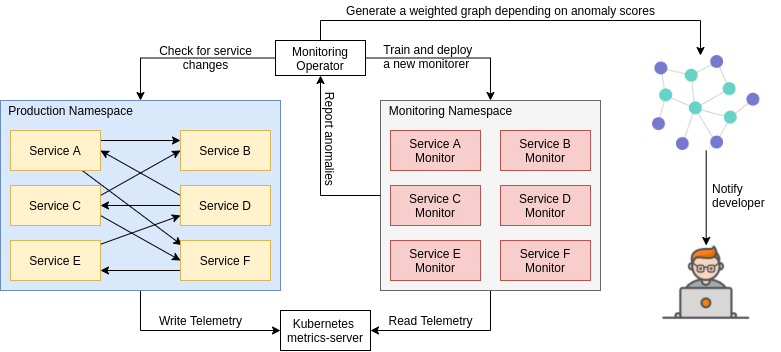
\includegraphics[width=16cm]{assets/High-level-system-diagram.png}
    \caption{Prototype feature diagram (self composed)}
    \label{fig:high-level-diagram}
\end{figure}
\section{Chapter Summary}

The above chapter described the participation of social, legal, ethical and professional issues in this project and how those were mitigated to comply with the BCS code of conduct.
\chapter{Introduction}
\pagenumbering{arabic}
\section{Chapter Overview}

The following chapter presents the evaluation process of this project and its findings. It starts by explaining the evaluation methodology and criteria for the project will be evaluated. The author then discusses their thoughts on the final product of this research. Then the thought process behind the selection evaluator will be explained. Finally, the chapter will conclude with feedback provided by the evaluators along with potential limitations in the evaluation.
\section{Problem Domain}

\subsection{Cloud Computing}
With an emergence of Infrastructure as a Services (IaaS) like Amazon Web Services (AWS) and Google Cloud Platform (GCP) there is a big surge in organizations trying to outsource their computing needs to third parties \citep{rimol_2021}. This is mainly due to the elasticity given by all the cloud providers. Users can easily scale up and down their infrastructures within minutes without making any commitment. All the major providers bill users on "what you use is what you pay model". Since the cloud provider manages all the underlying infrastructure, users doesn't have to worry about problems like hardware failures. In contrast in a self-hosted setting if the user wanted one extra GB of memory than what's available it requires a lot of effort and it cost a lot to full fill that requirement.

\subsection{Cloud-Native Applications}
During the 90s and early 2000s, all the applications were made as a big monolith from a single code base \citep{LessonsF52:online}. Most of them were shipped as a single binary. Since those days applications were fairly simple this worked very well with little to no downsides. When the 2010s came around there were a lot of specialized frameworks and programming languages and marketing teams wanted a lot of new futures quickly developed still maintaining reliability \citep{di2018migrating,Microser52:online}. But if the code base of the application was stored in a single repository, developers have to go through a long process to review and test if the changes won't break the current systems. Developers are also limited by the frameworks and programming languages that were chosen for the project at the start.

To tackle these problems a new way to develop applications was introduced, it's called "Microservices". The idea behind this concept is to break all the functionalities of big monolithic applications into small individually scalable services and give ownership of each service to small teams of people who work separately. With this flow developers are free to use whatever tool they like to develop each service. Because these services are developed parallelly by different teams this increases the development velocity by order of magnitude \citep{Understa56:online}.

As these services are relatively small and tailor-made to run on cloud environments it's easier to take something that's running on the developer's local machine to the production cluster in a matter of minutes. This is mainly thanks to modern cloud-native tools like CI/CD pipelines which automatically build and test the code for them, which can save a lot of time spent just doing repetitive tasks which are prone to human errors \citep{Whataret68:online}.

\subsection{Monitoring Cloud-Native Applications} \label{monitoring-bg}
Even though cloud-native applications have a lot to offer when it comes to developer velocity and productivity, It has its fair share of issues. Most of these problems are linked to the sheer complexity of these systems and not having a proper way to monitor them \citep{5WaysYou35:online}. All 3 major cloud providers provide a way to monitor these applications efficiently and there are some great open-source projects do this well, But to take full advantage of those systems, developers have to adapt their services to export all the vitals in a way the monitoring system understand. This works for the most part and this is what all the big companies are doing, even if it takes more developer time to in the end it's very crucial when it comes to disaster recovery.

But there is still a slight problem with this approach. Once the system starts to scale up to hundreds of services, the number vitals that has to be monitored goes to thousands and will require a lot of additional \acp{sres} and will have drop to lot of non-crucial service vitals and derive abstract \acp{sli} to make it \textbf{humanly} possible to understand what's going on.\\

\section{Problem Definition}

One of the leading problems in monitoring microservices is the sheer number of data that they generate. It's humanly impossible to monitor the metrics of all the services and it's hard for a single person to understand the entire system. By\acp{sres} using abstracted metrics called \acp{sli} which measures the quality of the service at a higher level can overcome this. Although \acp{sli} can alert when there is an issue in the system, it is difficult to understand where the actual problem is from this point on. To understand the root cause of the problem, \acp{sres} need to dig into \acp{apm} of all the services and go through each and every log of the troubling services.

When the system consists of hundreds or thousands of services that are interdependent; It is really hard to find where the actual issue is coming from and it may require the attention from all the service owners of the failing services to go through the logs and \acp{apm} to identify the actual root cause of the failure. This could greatly increase the \ac{mttr} and waste a lot of developer time by browsing logs.

\subsection{Problem Statement}

Modern distributed systems are becoming large and complex to the point where, when a failure occurs, it requires collaboration with a large number of people to find the actual root cause. Implementing a \textbf{framework} to make it easier to integrate machine learning models to detect anomalies in real-time could deflate \ac{mttr}.
\section{Existing Work}

\subsection{Anomaly detection}

\begin{longtable}{| p{20mm} | p{43mm} | p{43mm} | p{43mm} |}
\hline
  \textbf{Citation} &
  \textbf{Technology summary} &
  \textbf{Improvements} &
  \textbf{Limitations} \\ \hline


  \cite{du2018anomaly} &
  Tested most of common machine learning methods to detect anomalies and benchmarked them &
  \vspace{-8mm}
  \begin{itemize}[leftmargin=*,noitemsep,nolistsep] 
    \item Used \acp{sli} to monitored data
    \item A lot of good metrics (input data)
    \item Performance monitoring of services and containers
  \vspace{-7mm}
  \end{itemize} &
  \vspace{-8mm}
  \begin{itemize}[leftmargin=*,noitemsep,nolistsep] 
    \item Only be able to identify predetermined issues
    \item Require a sidecar that includes a lot of overheads
    \item Won't work with event-driven architectures (this is where most of the new systems are headed)
    \item Uses Supervised learning and it is nearly impossible to find real-world data with labels
  \vspace{-7mm}
  \end{itemize} \\ \hline


  \cite{kumarage2018anomaly} &
  The authors here propose a semi-supervised technique using a Variational Autoencoder to predict future time steps and calculate the difference between predicted and actual to detect anomalies. &
  \vspace{-8mm}
  \begin{itemize}[leftmargin=*,noitemsep,nolistsep] 
    \item Due to the difficulty of finding labelled research data, they settled on using a semi-supervised technique.
    \item Randomized decision trees used were used to select the most suitable characteristics for each component.
  \vspace{-7mm}
  \end{itemize} &
  \vspace{-8mm}
  \begin{itemize}[leftmargin=*,noitemsep,nolistsep] 
    \item The model will not be effortlessly transformable for other systems
    \item If more new key features were added to the system it will require a total retraining
  \vspace{-7mm}
  \end{itemize} \\ \hline


  \cite{kumarage2019generative} &
  Uses a bidirectional GAN to predict future timesteps and uses MSE between prediction and real to determine the anomalies &
  Experimented using a GAN to detect anomalies rather than using conventional autoencoders &
  \vspace{-8mm}
  \begin{itemize}[leftmargin=*,noitemsep,nolistsep] 
    \item Accuracy is around 60\%, which is unimpressive for use in production with mission-critical systems.
    \item As this is a GAN-based system, it may take numerous resources to run with production systems.
  \vspace{-7mm}
  \end{itemize} \\ \hline


  \caption{Comparison of anomaly detection methods in distributed systems (self-composed)}
\end{longtable}

\subsection{Root cause identification}

\begin{longtable}{| p{20mm} | p{40mm} | p{43mm} | p{46mm} |}
\hline
  \textbf{Citation} &
  \textbf{Technology summary} &
  \textbf{Improvements} &
  \textbf{Limitations} \\ \hline


  \cite{gonzalez2017root} &
  Detect failures in networks, using machine learning to generate knowledge graphs on historical data &
  \vspace{-8mm}
  \begin{itemize}[leftmargin=*,noitemsep,nolistsep] 
    \item Predictable system
    \item Automatic identification of dependencies between system events
    % \item independent of Domain experts
    \item Generalized to various systems
  \vspace{-7mm}
  \end{itemize} &
  \vspace{-8mm}
  \begin{itemize}[leftmargin=*,noitemsep,nolistsep] 
    \item Limited to network issues
    \item \acp{sres} must manually identify the issues, although the knowledge graph helped visualisation.
  \vspace{-7mm}
  \end{itemize} \\ \hline


  \cite{chigurupati2017root} &
  Proposed a way to detect hardware failures in servers using a probabilistic graphical model that concisely describes the relationship between many random variables and their conditional independence &
  \vspace{-8mm}
  \begin{itemize}[leftmargin=*,noitemsep,nolistsep] 
    \item Find hidden meaning in values that seems random
    \item Used a probabilistic approach to understand the relationship between inputs and outputs more clearly
    \item Gives all the possible root causes for a given problem
  \vspace{-7mm}
  \end{itemize} &
  \vspace{-8mm}
  \begin{itemize}[leftmargin=*,noitemsep,nolistsep] 
    \item Limited to hardware issues
    \item Require support from domain experts
    \item Can't account for unforeseen errors
  \vspace{-7mm}
  \end{itemize} \\ \hline


  \cite{wu2020microrca} &
  Find Performance bottlenecks in distributed systems using an attribute graph to find anomaly propagation across services and machines &
  \vspace{-8mm}
  \begin{itemize}[leftmargin=*,noitemsep,nolistsep] 
    \item Created a custom Fault Injection module
    \item Uses an attribute graph to localise to faulty service
    \item Application-agnostic by using a service mesh
    \item Rely on the service mesh to determine network topology
    \item Uses unsupervised learning
  \vspace{-7mm}
  \end{itemize} &
  \vspace{-8mm}
  \begin{itemize}[leftmargin=*,noitemsep,nolistsep] 
    \item Only able to identify 3 types of issues
    \item Checks only for performance anomalies
    \item Use the slow response time of a microservice as the definition of an anomaly
    \item Service meshes add a lot of overhead to systems
    \item Required direct connection between services
  \vspace{-7mm}
  \end{itemize} \\ \hline


  \cite{samir2019dla} &
  This detects and locates the anomalous behavior of microservices based on the observed response time using a HHMM &
  \vspace{-8mm}
  \begin{itemize}[leftmargin=*,noitemsep,nolistsep] 
    \item Custom HHMM model
    \item Self-healing mechanism
    \item Focus on performance detection and identification at the container, node, and service level
  \vspace{-7mm}
  \end{itemize} &
  \vspace{-8mm}
  \begin{itemize}[leftmargin=*,noitemsep,nolistsep] 
    \item The input data set scale is limited
    \item Require a sidecar
    \item Needs to predetermined thresholds
  \vspace{-7mm}
  \end{itemize} \\ \hline


  \caption{Comparison of root cause identification methods in distributed systems (self-composed)}
\end{longtable}

\subsection{Commercial products}

\begin{longtable}{| p{40mm} | p{55mm} | p{55mm} |}
\hline
  \textbf{Name} &
  \textbf{Futures} &
  \textbf{Limitations} \\ \hline


  Applied Intelligence by New Relic &
  \vspace{-8mm}
  \begin{itemize}[leftmargin=*,noitemsep,nolistsep] 
    \item Metric forecasting.
    \item Anomaly detection.
    \item Alert grouping to reduce noise.
  \vspace{-7mm}
  \end{itemize} &
  \vspace{-8mm}
  \begin{itemize}[leftmargin=*,noitemsep,nolistsep] 
    \item Lack of explanation for certain classifications.
    \item All the telemetry data need to be sent to a third party.
  \vspace{-7mm}
  \end{itemize} \\ \hline


  Watchdog by Datadog &
  \vspace{-8mm}
  \begin{itemize}[leftmargin=*,noitemsep,nolistsep] 
    \item Monitor the metric data of the entire system from the background.
    \item Monitor the log data.
    \item Highlight relevant components affected by an issue.
  \vspace{-7mm}
  \end{itemize} &
  \vspace{-8mm}
  \begin{itemize}[leftmargin=*,noitemsep,nolistsep] 
    \item Announced in 2018 but is still in private beta.
    \item Require code changes and tight integration with the datadog platform.
    \item Available demos about the system seem to be designed for demonstration purposes.
  \vspace{-7mm}
  \end{itemize} \\ \hline


  \caption{Comparison of commercial products for root cause analysis (self-composed)}
\end{longtable}
\section{The Novelty of the Research}

\subsection{Problem Novelty}

After a literature survey, the author concluded that finding the root cause of any failure within a distributed system is a challenging issue. This is mainly due to the fact that this problem cannot be assigned to a fixed set of inputs and outputs, which is a basic requirement for almost all types of neural network that are readily available. 

% Furthermore, almost all the researchers working on this problem domain have built their own solution for simulating a distributed system, since there isn't any open dataset on service monitoring. This could be mainly due to the fact that these datasets could contain sensitive information. 

Most of the currently established research was done towards creating statistical models like clustering and linear regression. Although these algorithms perform outstandingly in small-scale systems, they can struggle to adapt in the large-scale, noisy monitoring data found in medium-to large-sized systems. Another problem that was recognised was that none of these articles adequately addressed the issue of constant changes in services. Most published research considers target services static, but, in fact, these services can change constantly within a day \citep{GoingtoM51:online}. Finally, non of the published work has addressed the issue of scaling the anomaly detection system relative to the target distributed system which is a crucial factor for production use.

\subsection{Solution Novelty}


The focus of this project is to create an adaptable and scalable series of components that ranges from instrumentation to root cause analysis, which can be well integrated into an existing system or can be extended to fit to newer use cases. To achieve this the author is utilizing a fairly new technique called \ac{ebpf} for instrumentation, which is a Linux kernel API that can be used to track kernel events such as TCP socket changes to identify and understand the network layer of each application running on the system. Finally, for anomaly detection, a convolutional autoencoder with a novel data encoding method was used to keep the system as lightweight as possible, while still having acceptable accuracies for classifications. Combining that with a directed graph generated from collected network activity data can be used to highlight to blast radius of an anomaly along with possible causes.

\section{Research Question}


\begin{enumerate}[leftmargin=*,label=\textbf{RQ\arabic*:}]

\item How can a machine learning model improve \ac{mttr} in a distributed system?

\item What is the most efficient way to present raw data monitoring to machine learning model?

\item What will be the most ideal machine learning model to uncover anomalies in a microservice?

\item What are the methods that can be used to evaluate a root cause prediction system?

\end{enumerate}



\section{Research Motivation}

Modern distributed systems generate tons of useful and useless telemetry data. As the demand and size of the system increases, these telemetry data become more nosier and more complex \citep{Untangli35:online}. It makes difficult for humans to understand all these data, especially if they do not have long-standing experience with the system. On the other hand, deep learning models thrive when they have no end of data to learn from. As these models can be trained in computer-simulated environments, they can learn concepts that humans need years to grasp, within days \citep{OpenAI_dota, silver2017mastering}. Finally, unlike humans a deep learning model can monitor a service 24x7 without taking any breaks which will not only prevent outages even before they happen, It could be reduced \ac{mttr} because the issue can be detected way earlier than any human could do. 
\section{Research Challenge \& Potential}

% Even though this project seems very straightforward and easy to implement from a high level, it becomes problematic when it comes to reaching targets the author has set for himself. For an example, interpretability was one of the most requested features from the industry experts and a must-have trait for mission-critical systems \citep{ribeiro2016should}. But it was left out of the project scope due to its complexity especially when it comes to an undergraduate level project. Other than that following are a few of the more difficult challenges the author is expected to face while conducting the research.

\subsection{Research Challenge}

\begin{itemize}[leftmargin=*] 
    \item \textbf{Highly seasonal and noisy patterns} - Monitoring metrics on microservices in production tend to have very unpredictable patterns depending on the traffic that has been sent to the service. The amount of traffic sent will depend on several external factors that are hard to determine. Modeling both temporal dependencies and static interdependencies found in telemetry data of services into a single graph will be very difficult and require a lot of fine-tuning and data engineering skills.
    \item \textbf{Overhead} - Modern deep learning models can solve any problem if we could give them an unlimited amount of data and processing power. Although in this case, the models need to optimize for efficiency over accuracy since having a monitoring system that consumes a lot more resources than the actual target system isn't effective.
    \item \textbf{Fit into Kubernetes eco-system} - Kubernetes has become the de facto standard for managing distributed systems \citep{WhatisCo78:online}. So the author is planning to create a Kubernetes extension that will bridge the connection between monitored service and monitoring model. But Kubernetes itself has a very steep learning curve, even the original developers themselves have admitted that Kubernetes is too hard and complex for beginners \citep{Googlead4:online}.
    \item \textbf{Extraction of Telemetry} - Even though it's considered the best practice to implement telemetry exporting methods in the development phase of any application, developers often skip this part to save time. Sometimes it's required to depend on external applications that are developed by third parties which don't have means of exporting telemetry. Additionally, when building an end-to-end root course indication platform, it is required to take these kinds of scenario into account.
\end{itemize}

\subsection{Research Potential}

The feedback received for this project has been very positive because this is a very common but still unsolved issue in reliability engineering. Since this project was developed as a set of loosely coupled components, some of the experts expressed their interest in using individual components to solve some of the other problems they have been experiencing over time. Finally, this project can be used as an initial point for future research that focusses on specific areas of \ac{aiops} by replacing the individual components of this with their own.
\section{Research Aim}

\textit{The aim of this research is to design, develop and evaluate a low overhead Kubernetes framework to collect, store and process telemetry data using deep learning to help system operators detect anomalies earlier in order to reduce the \ac{mttr} when the system is experiencing an anomaly.}

In this project, the author tries to create a single model that can monitor all the vitals of a given service and output an anomaly score in any given time window. The author hopes to make it general enough so that operators can take the same model and deploy it with other services, and the model will be adopted to the new services using a few-shot learning method \citep{wang2020generalizing}. To make it happen, the author is trying to create a data encoding technique to represent monitoring data in a programming language/framework-independent way. To achieve this goal the author is also hoping to create a lightweight service instrumentation pipeline that can collect and process telemetry data in real-time without requiring any additional work from the user's end.
\section{Research Objectives}

\newcommand\robProblemIdentification{
When selecting the problem the author wanted to pursue, they had three main goals.
\begin{enumerate}[leftmargin=*,noitemsep,nolistsep,label=RO\arabic*:] 
    \item The problem domain should be something they would enjoy working on.
    \item At the end of the research they should give a meaningful impact to the target domain, both in the theoretical and practical aspect.
    \item It should be challenging to achieve, and the results should speak for themselves.
    \vspace{-7mm}
\end{enumerate}
}

\newcommand\robLiteratureReview{
Conduct a Literature review on root cause analysis, 
\begin{enumerate}[leftmargin=*,noitemsep,nolistsep,label=RO\arabic*:] 
    \setcounter{enumi}{3}
    \item To find the current methods that are used for anomaly detection and root cause localization.
    \item Uncover issues with current approaches.
    \item Understand how advancements in other related domains can apply to this domain.
    \vspace{-7mm}
\end{enumerate}
}


\newcommand\robDevelopingEvaluation{
During the literature survey, one of the problems the author identified was that there is no uniform data set when it comes to training or evaluating models to detect anomalies in microservices. Most of the researchers used private datasets to train and test their work.
To address this, the author is developing
\begin{enumerate}[leftmargin=*,noitemsep,nolistsep,label=RO\arabic*:] 
    \setcounter{enumi}{5}
    \item A tool that can easily simulate a distributed system in a cloud-native setting.
    \item A tool that can inject anomalies into the running services.
    \vspace{-7mm}
\end{enumerate}
}

\newcommand\robPublishPlayground{
The author hopes to publish a paper on the above-mentioned tool so that future researchers will have a unified way to train, test, and benchmark their system without having to reinvent the wheel again and again.
}

\newcommand\robDataGathering{
To create a model to detect anomalies, the author will have to
\begin{enumerate}[leftmargin=15mm,noitemsep,nolistsep,label=RO\arabic*:] 
    \setcounter{enumi}{7}
    \item Simulate a distributed system.
    \item Simulate the traffic inside the system.
    \item Collect monitoring data while it's running.
    \vspace{-7mm}
\end{enumerate}
}

\newcommand\robDevelopingEncoding{
Since these microservices will report very different metric values even at idle depending on the architecture of the service. To normalize theses data points from all the services to one format author will,
\begin{enumerate}[leftmargin=15mm,noitemsep,nolistsep,label=RO\arabic*:] 
    \setcounter{enumi}{10}
    \item Evaluate current data encoding methods such as \cite{zhang2019deep}.
    \item Find the best fit and optimise it for this use case.
    \item Test if there is improvement by using that method. 
    \vspace{-7mm}
\end{enumerate}
}


\newcommand\robDevelopingModel{
According to \cite{kumarage2019generative}, autoencoders tend to perform best when it comes to anomaly detection. But during the literature survey it was revealed that convolution autoencoders weren't tested for this usecase. So, the author is hoping to develop a convolution auto-encoder and test how it will perform.
}


\newcommand\robTesting{
The following things will be tested during the testing phase, 
\begin{enumerate}[leftmargin=15mm,noitemsep,nolistsep,label=RO\arabic*:] 
    \setcounter{enumi}{13}
    \item How will the system classify long-term \& short-term fluctuations.
    \item What will be the overhead of the system.
    \item Can the system understand the mapping between core metrics like CPU and Memory usages.
    \item Accuracy of fault detection.
    \item Reliability of the instrumentation system.
\vspace{-7mm}
\end{enumerate}
}

\newcommand\robIntegration{
Having a fancy model does not add anything if it is very hard to use with a real system. So the author is hoping to develop a Kubernetes extension that will map the model with any service given by the user.
}


\begin{longtable}{|p{20mm}|p{90mm}|p{19mm}|p{17mm}|}
\hline
    \textbf{Research Objectives} &
    \textbf{Explanation} &
    \textbf{Learning Outcomes} &
    \textbf{Research Questions} \\ \hline

    Problem identification &
    \robProblemIdentification &
    LO1 &
    RQ1, RQ3 \\ \hline

    Literature review &
    \robLiteratureReview &
    LO3, LO4, LO6 &
    RQ1, RQ2, RQ3, RQ4 \\ \hline

    Developing an evaluation framework &
    \robDevelopingEvaluation &
    LO7 &
    RQ4 \\ \hline

    % Publish a paper on that playground &
    % \robPublishPlayground &
    % LO7 &
    % N/A \\ \hline

    Data gathering and analysis &
    \robDataGathering &
    LO7 &
    RQ2, RQ4 \\ \hline

    Developing the encoding method &
    \robDevelopingEncoding &
    LO2, LO5, LO7 &
    RQ2, RQ3 \\ \hline

    Developing the model &
    \robDevelopingModel &
    LO2, LO5, LO7 &
    RQ4 \\ \hline

    Testing and evaluation &
    \robTesting &
    LO8, LO9 &
    RQ1, RQ3, RQ4 \\ \hline

    Integration &
    \robIntegration &
    LO7 &
    RQ1, RQ3 \\ \hline

\caption{Research Objectives (self-composed)}
\end{longtable}

\section{Research Contribution}


\subsection{Domain Contribution}

With this research, the author first tried to develop a \textbf{cloud-native solution to create a configurable microservices system}, so this research and future research will have a standard environment to develop and evaluate their work. The author built a lightweight and \textbf{low-overhead data collection pipeline} using \ac{ebpf} to collect telemetry of target services without any instrumentation from the user.

\subsection{Knowledge Contribution}

One of the main problems with monitoring microservices systems is that different services can be developed with different programming languages and frameworks, and those can contain different levels of noise\label{need-for-encoding}. Therefore, it is complicated for a single model to detect anomalies in any service since some frameworks tend to use more resources while idle than others. To address this author is trying to come up with an \textbf{encoding method} so the model can be trained to monitor one framework and those learning will still be valid for another framework. With these encoded data, the author is hoping to develop a \textbf{convolutional autoencoder that will use unsupervised learning to spot out anomalies in a given data stream}. This may have better performance while using fewer resources since convolutional layers are typically lightweight and good at pattern recognition \citep{oord2016wavenet}. Finally, the author plans to aggregate these predictions from the models into a pre-generated service graph and weigh them at \textbf{find all possible root causes}.

{\let\clearpage\relax\chapter{Project Scope}}

From the literature survey and talking with industry, experts author found many issues they can address when developing the system, but some of those problems like interpretability on autoencoder \citep{ribeiro2016should} are hard to solve by someone at a level of an undergraduate. As this project is done by one developer in less than one year, it won't be possible to create a fully functional monitoring platform like Datadog or New Relic. The Force of this project is to see if the author can develop a single model that can monitor all kinds of services after transfer learning with few examples. \\

\newpage

\section{In-scope} \label{sec:in-scope}
Following are the main forces of this project
\begin{itemize}[noitemsep,nolistsep] 
    \item Evaluation Framework
    \begin{itemize}[noitemsep,nolistsep] 
        \item Ability to create service mesh out using Kubernetes native resources.
        \item Each service has the ability to simulator predefined error types.
        \item Service mesh can be made up of services written in different programming languages and  frameworks.
        \item Built-in method to run stress tests.
    \end{itemize}
    \item Monitoring System
    \begin{itemize}[noitemsep,nolistsep]
        \item Low overhead data collection pipeline to collect service telemetry.
        \item Reliability system which generate fewer false positives so it won't overwhelm the operators and false negatives will be caught by the main monitoring system.
        \item Optimized models to have fairly small memory footprint and a CPU overhead.
        \item Well generalized model which will be able to deploy with completely new services and it will learn to adapt the new system.
    \end{itemize}
\end{itemize}


% \item Constant changes to services
% \item Highly seasonal and noisy patterns 
% \item few shot learning to convert to a new system
% \item Tunability
% \item Reponsed to seasonal dependencies 
% \end{enumerate}



\section{Out-scope} \label{sec:out-scope}
Follow will not be covered during this project
\begin{itemize}[noitemsep,nolistsep] 
    \item Evaluation Framework
    \begin{itemize}[noitemsep,nolistsep] 
        \item Support for every major language and framework.
        \item Working outside of Kubernetes eco-system.
    \end{itemize}
    \item Monitoring System
    \begin{itemize}[noitemsep,nolistsep] 
        \item Interpretability - Describing a behavior of autoencoder is a difficult task that won't be covered during the project.
        \item System won't be trained against data from a real production system due to the lack of public datasets.
        \item System won't have very high accuracy, as this will be the first line of defense this will try to avoid false positives to prevent adding more noise to alerting systems.
        \item Automatically identify system topology.
        \item This will not be a drop-in replacement for existing monitoring systems, rather this will work with existing monitoring systems to reduce the \ac{mttr}.
    \end{itemize}
\end{itemize}

\section{Prototype Feature Diagram}
\begin{figure}[H]
    \centering
    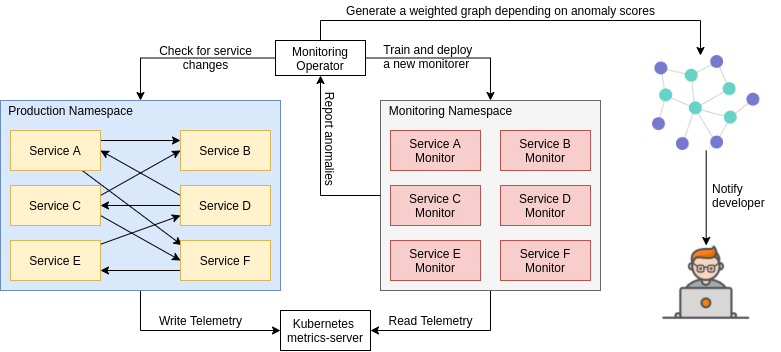
\includegraphics[width=16cm]{assets/High-level-system-diagram.png}
    \caption{Prototype feature diagram (self composed)}
    \label{fig:high-level-diagram}
\end{figure}
\section{Chapter Summary}

The above chapter described the participation of social, legal, ethical and professional issues in this project and how those were mitigated to comply with the BCS code of conduct.
\chapter{Introduction}
\pagenumbering{arabic}
\section{Chapter Overview}

The following chapter presents the evaluation process of this project and its findings. It starts by explaining the evaluation methodology and criteria for the project will be evaluated. The author then discusses their thoughts on the final product of this research. Then the thought process behind the selection evaluator will be explained. Finally, the chapter will conclude with feedback provided by the evaluators along with potential limitations in the evaluation.
\section{Problem Domain}

\subsection{Cloud Computing}
With an emergence of Infrastructure as a Services (IaaS) like Amazon Web Services (AWS) and Google Cloud Platform (GCP) there is a big surge in organizations trying to outsource their computing needs to third parties \citep{rimol_2021}. This is mainly due to the elasticity given by all the cloud providers. Users can easily scale up and down their infrastructures within minutes without making any commitment. All the major providers bill users on "what you use is what you pay model". Since the cloud provider manages all the underlying infrastructure, users doesn't have to worry about problems like hardware failures. In contrast in a self-hosted setting if the user wanted one extra GB of memory than what's available it requires a lot of effort and it cost a lot to full fill that requirement.

\subsection{Cloud-Native Applications}
During the 90s and early 2000s, all the applications were made as a big monolith from a single code base \citep{LessonsF52:online}. Most of them were shipped as a single binary. Since those days applications were fairly simple this worked very well with little to no downsides. When the 2010s came around there were a lot of specialized frameworks and programming languages and marketing teams wanted a lot of new futures quickly developed still maintaining reliability \citep{di2018migrating,Microser52:online}. But if the code base of the application was stored in a single repository, developers have to go through a long process to review and test if the changes won't break the current systems. Developers are also limited by the frameworks and programming languages that were chosen for the project at the start.

To tackle these problems a new way to develop applications was introduced, it's called "Microservices". The idea behind this concept is to break all the functionalities of big monolithic applications into small individually scalable services and give ownership of each service to small teams of people who work separately. With this flow developers are free to use whatever tool they like to develop each service. Because these services are developed parallelly by different teams this increases the development velocity by order of magnitude \citep{Understa56:online}.

As these services are relatively small and tailor-made to run on cloud environments it's easier to take something that's running on the developer's local machine to the production cluster in a matter of minutes. This is mainly thanks to modern cloud-native tools like CI/CD pipelines which automatically build and test the code for them, which can save a lot of time spent just doing repetitive tasks which are prone to human errors \citep{Whataret68:online}.

\subsection{Monitoring Cloud-Native Applications} \label{monitoring-bg}
Even though cloud-native applications have a lot to offer when it comes to developer velocity and productivity, It has its fair share of issues. Most of these problems are linked to the sheer complexity of these systems and not having a proper way to monitor them \citep{5WaysYou35:online}. All 3 major cloud providers provide a way to monitor these applications efficiently and there are some great open-source projects do this well, But to take full advantage of those systems, developers have to adapt their services to export all the vitals in a way the monitoring system understand. This works for the most part and this is what all the big companies are doing, even if it takes more developer time to in the end it's very crucial when it comes to disaster recovery.

But there is still a slight problem with this approach. Once the system starts to scale up to hundreds of services, the number vitals that has to be monitored goes to thousands and will require a lot of additional \acp{sres} and will have drop to lot of non-crucial service vitals and derive abstract \acp{sli} to make it \textbf{humanly} possible to understand what's going on.\\

\section{Problem Definition}

One of the leading problems in monitoring microservices is the sheer number of data that they generate. It's humanly impossible to monitor the metrics of all the services and it's hard for a single person to understand the entire system. By\acp{sres} using abstracted metrics called \acp{sli} which measures the quality of the service at a higher level can overcome this. Although \acp{sli} can alert when there is an issue in the system, it is difficult to understand where the actual problem is from this point on. To understand the root cause of the problem, \acp{sres} need to dig into \acp{apm} of all the services and go through each and every log of the troubling services.

When the system consists of hundreds or thousands of services that are interdependent; It is really hard to find where the actual issue is coming from and it may require the attention from all the service owners of the failing services to go through the logs and \acp{apm} to identify the actual root cause of the failure. This could greatly increase the \ac{mttr} and waste a lot of developer time by browsing logs.

\subsection{Problem Statement}

Modern distributed systems are becoming large and complex to the point where, when a failure occurs, it requires collaboration with a large number of people to find the actual root cause. Implementing a \textbf{framework} to make it easier to integrate machine learning models to detect anomalies in real-time could deflate \ac{mttr}.
\section{Existing Work}

\subsection{Anomaly detection}

\begin{longtable}{| p{20mm} | p{43mm} | p{43mm} | p{43mm} |}
\hline
  \textbf{Citation} &
  \textbf{Technology summary} &
  \textbf{Improvements} &
  \textbf{Limitations} \\ \hline


  \cite{du2018anomaly} &
  Tested most of common machine learning methods to detect anomalies and benchmarked them &
  \vspace{-8mm}
  \begin{itemize}[leftmargin=*,noitemsep,nolistsep] 
    \item Used \acp{sli} to monitored data
    \item A lot of good metrics (input data)
    \item Performance monitoring of services and containers
  \vspace{-7mm}
  \end{itemize} &
  \vspace{-8mm}
  \begin{itemize}[leftmargin=*,noitemsep,nolistsep] 
    \item Only be able to identify predetermined issues
    \item Require a sidecar that includes a lot of overheads
    \item Won't work with event-driven architectures (this is where most of the new systems are headed)
    \item Uses Supervised learning and it is nearly impossible to find real-world data with labels
  \vspace{-7mm}
  \end{itemize} \\ \hline


  \cite{kumarage2018anomaly} &
  The authors here propose a semi-supervised technique using a Variational Autoencoder to predict future time steps and calculate the difference between predicted and actual to detect anomalies. &
  \vspace{-8mm}
  \begin{itemize}[leftmargin=*,noitemsep,nolistsep] 
    \item Due to the difficulty of finding labelled research data, they settled on using a semi-supervised technique.
    \item Randomized decision trees used were used to select the most suitable characteristics for each component.
  \vspace{-7mm}
  \end{itemize} &
  \vspace{-8mm}
  \begin{itemize}[leftmargin=*,noitemsep,nolistsep] 
    \item The model will not be effortlessly transformable for other systems
    \item If more new key features were added to the system it will require a total retraining
  \vspace{-7mm}
  \end{itemize} \\ \hline


  \cite{kumarage2019generative} &
  Uses a bidirectional GAN to predict future timesteps and uses MSE between prediction and real to determine the anomalies &
  Experimented using a GAN to detect anomalies rather than using conventional autoencoders &
  \vspace{-8mm}
  \begin{itemize}[leftmargin=*,noitemsep,nolistsep] 
    \item Accuracy is around 60\%, which is unimpressive for use in production with mission-critical systems.
    \item As this is a GAN-based system, it may take numerous resources to run with production systems.
  \vspace{-7mm}
  \end{itemize} \\ \hline


  \caption{Comparison of anomaly detection methods in distributed systems (self-composed)}
\end{longtable}

\subsection{Root cause identification}

\begin{longtable}{| p{20mm} | p{40mm} | p{43mm} | p{46mm} |}
\hline
  \textbf{Citation} &
  \textbf{Technology summary} &
  \textbf{Improvements} &
  \textbf{Limitations} \\ \hline


  \cite{gonzalez2017root} &
  Detect failures in networks, using machine learning to generate knowledge graphs on historical data &
  \vspace{-8mm}
  \begin{itemize}[leftmargin=*,noitemsep,nolistsep] 
    \item Predictable system
    \item Automatic identification of dependencies between system events
    % \item independent of Domain experts
    \item Generalized to various systems
  \vspace{-7mm}
  \end{itemize} &
  \vspace{-8mm}
  \begin{itemize}[leftmargin=*,noitemsep,nolistsep] 
    \item Limited to network issues
    \item \acp{sres} must manually identify the issues, although the knowledge graph helped visualisation.
  \vspace{-7mm}
  \end{itemize} \\ \hline


  \cite{chigurupati2017root} &
  Proposed a way to detect hardware failures in servers using a probabilistic graphical model that concisely describes the relationship between many random variables and their conditional independence &
  \vspace{-8mm}
  \begin{itemize}[leftmargin=*,noitemsep,nolistsep] 
    \item Find hidden meaning in values that seems random
    \item Used a probabilistic approach to understand the relationship between inputs and outputs more clearly
    \item Gives all the possible root causes for a given problem
  \vspace{-7mm}
  \end{itemize} &
  \vspace{-8mm}
  \begin{itemize}[leftmargin=*,noitemsep,nolistsep] 
    \item Limited to hardware issues
    \item Require support from domain experts
    \item Can't account for unforeseen errors
  \vspace{-7mm}
  \end{itemize} \\ \hline


  \cite{wu2020microrca} &
  Find Performance bottlenecks in distributed systems using an attribute graph to find anomaly propagation across services and machines &
  \vspace{-8mm}
  \begin{itemize}[leftmargin=*,noitemsep,nolistsep] 
    \item Created a custom Fault Injection module
    \item Uses an attribute graph to localise to faulty service
    \item Application-agnostic by using a service mesh
    \item Rely on the service mesh to determine network topology
    \item Uses unsupervised learning
  \vspace{-7mm}
  \end{itemize} &
  \vspace{-8mm}
  \begin{itemize}[leftmargin=*,noitemsep,nolistsep] 
    \item Only able to identify 3 types of issues
    \item Checks only for performance anomalies
    \item Use the slow response time of a microservice as the definition of an anomaly
    \item Service meshes add a lot of overhead to systems
    \item Required direct connection between services
  \vspace{-7mm}
  \end{itemize} \\ \hline


  \cite{samir2019dla} &
  This detects and locates the anomalous behavior of microservices based on the observed response time using a HHMM &
  \vspace{-8mm}
  \begin{itemize}[leftmargin=*,noitemsep,nolistsep] 
    \item Custom HHMM model
    \item Self-healing mechanism
    \item Focus on performance detection and identification at the container, node, and service level
  \vspace{-7mm}
  \end{itemize} &
  \vspace{-8mm}
  \begin{itemize}[leftmargin=*,noitemsep,nolistsep] 
    \item The input data set scale is limited
    \item Require a sidecar
    \item Needs to predetermined thresholds
  \vspace{-7mm}
  \end{itemize} \\ \hline


  \caption{Comparison of root cause identification methods in distributed systems (self-composed)}
\end{longtable}

\subsection{Commercial products}

\begin{longtable}{| p{40mm} | p{55mm} | p{55mm} |}
\hline
  \textbf{Name} &
  \textbf{Futures} &
  \textbf{Limitations} \\ \hline


  Applied Intelligence by New Relic &
  \vspace{-8mm}
  \begin{itemize}[leftmargin=*,noitemsep,nolistsep] 
    \item Metric forecasting.
    \item Anomaly detection.
    \item Alert grouping to reduce noise.
  \vspace{-7mm}
  \end{itemize} &
  \vspace{-8mm}
  \begin{itemize}[leftmargin=*,noitemsep,nolistsep] 
    \item Lack of explanation for certain classifications.
    \item All the telemetry data need to be sent to a third party.
  \vspace{-7mm}
  \end{itemize} \\ \hline


  Watchdog by Datadog &
  \vspace{-8mm}
  \begin{itemize}[leftmargin=*,noitemsep,nolistsep] 
    \item Monitor the metric data of the entire system from the background.
    \item Monitor the log data.
    \item Highlight relevant components affected by an issue.
  \vspace{-7mm}
  \end{itemize} &
  \vspace{-8mm}
  \begin{itemize}[leftmargin=*,noitemsep,nolistsep] 
    \item Announced in 2018 but is still in private beta.
    \item Require code changes and tight integration with the datadog platform.
    \item Available demos about the system seem to be designed for demonstration purposes.
  \vspace{-7mm}
  \end{itemize} \\ \hline


  \caption{Comparison of commercial products for root cause analysis (self-composed)}
\end{longtable}
\section{The Novelty of the Research}

\subsection{Problem Novelty}

After a literature survey, the author concluded that finding the root cause of any failure within a distributed system is a challenging issue. This is mainly due to the fact that this problem cannot be assigned to a fixed set of inputs and outputs, which is a basic requirement for almost all types of neural network that are readily available. 

% Furthermore, almost all the researchers working on this problem domain have built their own solution for simulating a distributed system, since there isn't any open dataset on service monitoring. This could be mainly due to the fact that these datasets could contain sensitive information. 

Most of the currently established research was done towards creating statistical models like clustering and linear regression. Although these algorithms perform outstandingly in small-scale systems, they can struggle to adapt in the large-scale, noisy monitoring data found in medium-to large-sized systems. Another problem that was recognised was that none of these articles adequately addressed the issue of constant changes in services. Most published research considers target services static, but, in fact, these services can change constantly within a day \citep{GoingtoM51:online}. Finally, non of the published work has addressed the issue of scaling the anomaly detection system relative to the target distributed system which is a crucial factor for production use.

\subsection{Solution Novelty}


The focus of this project is to create an adaptable and scalable series of components that ranges from instrumentation to root cause analysis, which can be well integrated into an existing system or can be extended to fit to newer use cases. To achieve this the author is utilizing a fairly new technique called \ac{ebpf} for instrumentation, which is a Linux kernel API that can be used to track kernel events such as TCP socket changes to identify and understand the network layer of each application running on the system. Finally, for anomaly detection, a convolutional autoencoder with a novel data encoding method was used to keep the system as lightweight as possible, while still having acceptable accuracies for classifications. Combining that with a directed graph generated from collected network activity data can be used to highlight to blast radius of an anomaly along with possible causes.

\section{Research Question}


\begin{enumerate}[leftmargin=*,label=\textbf{RQ\arabic*:}]

\item How can a machine learning model improve \ac{mttr} in a distributed system?

\item What is the most efficient way to present raw data monitoring to machine learning model?

\item What will be the most ideal machine learning model to uncover anomalies in a microservice?

\item What are the methods that can be used to evaluate a root cause prediction system?

\end{enumerate}



\section{Research Motivation}

Modern distributed systems generate tons of useful and useless telemetry data. As the demand and size of the system increases, these telemetry data become more nosier and more complex \citep{Untangli35:online}. It makes difficult for humans to understand all these data, especially if they do not have long-standing experience with the system. On the other hand, deep learning models thrive when they have no end of data to learn from. As these models can be trained in computer-simulated environments, they can learn concepts that humans need years to grasp, within days \citep{OpenAI_dota, silver2017mastering}. Finally, unlike humans a deep learning model can monitor a service 24x7 without taking any breaks which will not only prevent outages even before they happen, It could be reduced \ac{mttr} because the issue can be detected way earlier than any human could do. 
\section{Research Challenge \& Potential}

% Even though this project seems very straightforward and easy to implement from a high level, it becomes problematic when it comes to reaching targets the author has set for himself. For an example, interpretability was one of the most requested features from the industry experts and a must-have trait for mission-critical systems \citep{ribeiro2016should}. But it was left out of the project scope due to its complexity especially when it comes to an undergraduate level project. Other than that following are a few of the more difficult challenges the author is expected to face while conducting the research.

\subsection{Research Challenge}

\begin{itemize}[leftmargin=*] 
    \item \textbf{Highly seasonal and noisy patterns} - Monitoring metrics on microservices in production tend to have very unpredictable patterns depending on the traffic that has been sent to the service. The amount of traffic sent will depend on several external factors that are hard to determine. Modeling both temporal dependencies and static interdependencies found in telemetry data of services into a single graph will be very difficult and require a lot of fine-tuning and data engineering skills.
    \item \textbf{Overhead} - Modern deep learning models can solve any problem if we could give them an unlimited amount of data and processing power. Although in this case, the models need to optimize for efficiency over accuracy since having a monitoring system that consumes a lot more resources than the actual target system isn't effective.
    \item \textbf{Fit into Kubernetes eco-system} - Kubernetes has become the de facto standard for managing distributed systems \citep{WhatisCo78:online}. So the author is planning to create a Kubernetes extension that will bridge the connection between monitored service and monitoring model. But Kubernetes itself has a very steep learning curve, even the original developers themselves have admitted that Kubernetes is too hard and complex for beginners \citep{Googlead4:online}.
    \item \textbf{Extraction of Telemetry} - Even though it's considered the best practice to implement telemetry exporting methods in the development phase of any application, developers often skip this part to save time. Sometimes it's required to depend on external applications that are developed by third parties which don't have means of exporting telemetry. Additionally, when building an end-to-end root course indication platform, it is required to take these kinds of scenario into account.
\end{itemize}

\subsection{Research Potential}

The feedback received for this project has been very positive because this is a very common but still unsolved issue in reliability engineering. Since this project was developed as a set of loosely coupled components, some of the experts expressed their interest in using individual components to solve some of the other problems they have been experiencing over time. Finally, this project can be used as an initial point for future research that focusses on specific areas of \ac{aiops} by replacing the individual components of this with their own.
\section{Research Aim}

\textit{The aim of this research is to design, develop and evaluate a low overhead Kubernetes framework to collect, store and process telemetry data using deep learning to help system operators detect anomalies earlier in order to reduce the \ac{mttr} when the system is experiencing an anomaly.}

In this project, the author tries to create a single model that can monitor all the vitals of a given service and output an anomaly score in any given time window. The author hopes to make it general enough so that operators can take the same model and deploy it with other services, and the model will be adopted to the new services using a few-shot learning method \citep{wang2020generalizing}. To make it happen, the author is trying to create a data encoding technique to represent monitoring data in a programming language/framework-independent way. To achieve this goal the author is also hoping to create a lightweight service instrumentation pipeline that can collect and process telemetry data in real-time without requiring any additional work from the user's end.
\section{Research Objectives}

\newcommand\robProblemIdentification{
When selecting the problem the author wanted to pursue, they had three main goals.
\begin{enumerate}[leftmargin=*,noitemsep,nolistsep,label=RO\arabic*:] 
    \item The problem domain should be something they would enjoy working on.
    \item At the end of the research they should give a meaningful impact to the target domain, both in the theoretical and practical aspect.
    \item It should be challenging to achieve, and the results should speak for themselves.
    \vspace{-7mm}
\end{enumerate}
}

\newcommand\robLiteratureReview{
Conduct a Literature review on root cause analysis, 
\begin{enumerate}[leftmargin=*,noitemsep,nolistsep,label=RO\arabic*:] 
    \setcounter{enumi}{3}
    \item To find the current methods that are used for anomaly detection and root cause localization.
    \item Uncover issues with current approaches.
    \item Understand how advancements in other related domains can apply to this domain.
    \vspace{-7mm}
\end{enumerate}
}


\newcommand\robDevelopingEvaluation{
During the literature survey, one of the problems the author identified was that there is no uniform data set when it comes to training or evaluating models to detect anomalies in microservices. Most of the researchers used private datasets to train and test their work.
To address this, the author is developing
\begin{enumerate}[leftmargin=*,noitemsep,nolistsep,label=RO\arabic*:] 
    \setcounter{enumi}{5}
    \item A tool that can easily simulate a distributed system in a cloud-native setting.
    \item A tool that can inject anomalies into the running services.
    \vspace{-7mm}
\end{enumerate}
}

\newcommand\robPublishPlayground{
The author hopes to publish a paper on the above-mentioned tool so that future researchers will have a unified way to train, test, and benchmark their system without having to reinvent the wheel again and again.
}

\newcommand\robDataGathering{
To create a model to detect anomalies, the author will have to
\begin{enumerate}[leftmargin=15mm,noitemsep,nolistsep,label=RO\arabic*:] 
    \setcounter{enumi}{7}
    \item Simulate a distributed system.
    \item Simulate the traffic inside the system.
    \item Collect monitoring data while it's running.
    \vspace{-7mm}
\end{enumerate}
}

\newcommand\robDevelopingEncoding{
Since these microservices will report very different metric values even at idle depending on the architecture of the service. To normalize theses data points from all the services to one format author will,
\begin{enumerate}[leftmargin=15mm,noitemsep,nolistsep,label=RO\arabic*:] 
    \setcounter{enumi}{10}
    \item Evaluate current data encoding methods such as \cite{zhang2019deep}.
    \item Find the best fit and optimise it for this use case.
    \item Test if there is improvement by using that method. 
    \vspace{-7mm}
\end{enumerate}
}


\newcommand\robDevelopingModel{
According to \cite{kumarage2019generative}, autoencoders tend to perform best when it comes to anomaly detection. But during the literature survey it was revealed that convolution autoencoders weren't tested for this usecase. So, the author is hoping to develop a convolution auto-encoder and test how it will perform.
}


\newcommand\robTesting{
The following things will be tested during the testing phase, 
\begin{enumerate}[leftmargin=15mm,noitemsep,nolistsep,label=RO\arabic*:] 
    \setcounter{enumi}{13}
    \item How will the system classify long-term \& short-term fluctuations.
    \item What will be the overhead of the system.
    \item Can the system understand the mapping between core metrics like CPU and Memory usages.
    \item Accuracy of fault detection.
    \item Reliability of the instrumentation system.
\vspace{-7mm}
\end{enumerate}
}

\newcommand\robIntegration{
Having a fancy model does not add anything if it is very hard to use with a real system. So the author is hoping to develop a Kubernetes extension that will map the model with any service given by the user.
}


\begin{longtable}{|p{20mm}|p{90mm}|p{19mm}|p{17mm}|}
\hline
    \textbf{Research Objectives} &
    \textbf{Explanation} &
    \textbf{Learning Outcomes} &
    \textbf{Research Questions} \\ \hline

    Problem identification &
    \robProblemIdentification &
    LO1 &
    RQ1, RQ3 \\ \hline

    Literature review &
    \robLiteratureReview &
    LO3, LO4, LO6 &
    RQ1, RQ2, RQ3, RQ4 \\ \hline

    Developing an evaluation framework &
    \robDevelopingEvaluation &
    LO7 &
    RQ4 \\ \hline

    % Publish a paper on that playground &
    % \robPublishPlayground &
    % LO7 &
    % N/A \\ \hline

    Data gathering and analysis &
    \robDataGathering &
    LO7 &
    RQ2, RQ4 \\ \hline

    Developing the encoding method &
    \robDevelopingEncoding &
    LO2, LO5, LO7 &
    RQ2, RQ3 \\ \hline

    Developing the model &
    \robDevelopingModel &
    LO2, LO5, LO7 &
    RQ4 \\ \hline

    Testing and evaluation &
    \robTesting &
    LO8, LO9 &
    RQ1, RQ3, RQ4 \\ \hline

    Integration &
    \robIntegration &
    LO7 &
    RQ1, RQ3 \\ \hline

\caption{Research Objectives (self-composed)}
\end{longtable}

\section{Research Contribution}


\subsection{Domain Contribution}

With this research, the author first tried to develop a \textbf{cloud-native solution to create a configurable microservices system}, so this research and future research will have a standard environment to develop and evaluate their work. The author built a lightweight and \textbf{low-overhead data collection pipeline} using \ac{ebpf} to collect telemetry of target services without any instrumentation from the user.

\subsection{Knowledge Contribution}

One of the main problems with monitoring microservices systems is that different services can be developed with different programming languages and frameworks, and those can contain different levels of noise\label{need-for-encoding}. Therefore, it is complicated for a single model to detect anomalies in any service since some frameworks tend to use more resources while idle than others. To address this author is trying to come up with an \textbf{encoding method} so the model can be trained to monitor one framework and those learning will still be valid for another framework. With these encoded data, the author is hoping to develop a \textbf{convolutional autoencoder that will use unsupervised learning to spot out anomalies in a given data stream}. This may have better performance while using fewer resources since convolutional layers are typically lightweight and good at pattern recognition \citep{oord2016wavenet}. Finally, the author plans to aggregate these predictions from the models into a pre-generated service graph and weigh them at \textbf{find all possible root causes}.

{\let\clearpage\relax\chapter{Project Scope}}

From the literature survey and talking with industry, experts author found many issues they can address when developing the system, but some of those problems like interpretability on autoencoder \citep{ribeiro2016should} are hard to solve by someone at a level of an undergraduate. As this project is done by one developer in less than one year, it won't be possible to create a fully functional monitoring platform like Datadog or New Relic. The Force of this project is to see if the author can develop a single model that can monitor all kinds of services after transfer learning with few examples. \\

\newpage

\section{In-scope} \label{sec:in-scope}
Following are the main forces of this project
\begin{itemize}[noitemsep,nolistsep] 
    \item Evaluation Framework
    \begin{itemize}[noitemsep,nolistsep] 
        \item Ability to create service mesh out using Kubernetes native resources.
        \item Each service has the ability to simulator predefined error types.
        \item Service mesh can be made up of services written in different programming languages and  frameworks.
        \item Built-in method to run stress tests.
    \end{itemize}
    \item Monitoring System
    \begin{itemize}[noitemsep,nolistsep]
        \item Low overhead data collection pipeline to collect service telemetry.
        \item Reliability system which generate fewer false positives so it won't overwhelm the operators and false negatives will be caught by the main monitoring system.
        \item Optimized models to have fairly small memory footprint and a CPU overhead.
        \item Well generalized model which will be able to deploy with completely new services and it will learn to adapt the new system.
    \end{itemize}
\end{itemize}


% \item Constant changes to services
% \item Highly seasonal and noisy patterns 
% \item few shot learning to convert to a new system
% \item Tunability
% \item Reponsed to seasonal dependencies 
% \end{enumerate}



\section{Out-scope} \label{sec:out-scope}
Follow will not be covered during this project
\begin{itemize}[noitemsep,nolistsep] 
    \item Evaluation Framework
    \begin{itemize}[noitemsep,nolistsep] 
        \item Support for every major language and framework.
        \item Working outside of Kubernetes eco-system.
    \end{itemize}
    \item Monitoring System
    \begin{itemize}[noitemsep,nolistsep] 
        \item Interpretability - Describing a behavior of autoencoder is a difficult task that won't be covered during the project.
        \item System won't be trained against data from a real production system due to the lack of public datasets.
        \item System won't have very high accuracy, as this will be the first line of defense this will try to avoid false positives to prevent adding more noise to alerting systems.
        \item Automatically identify system topology.
        \item This will not be a drop-in replacement for existing monitoring systems, rather this will work with existing monitoring systems to reduce the \ac{mttr}.
    \end{itemize}
\end{itemize}

\section{Prototype Feature Diagram}
\begin{figure}[H]
    \centering
    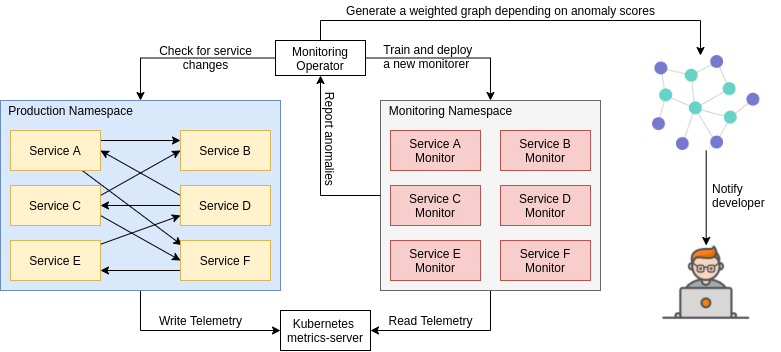
\includegraphics[width=16cm]{assets/High-level-system-diagram.png}
    \caption{Prototype feature diagram (self composed)}
    \label{fig:high-level-diagram}
\end{figure}
\section{Chapter Summary}

The above chapter described the participation of social, legal, ethical and professional issues in this project and how those were mitigated to comply with the BCS code of conduct.

\cleardoublepage
\phantomsection
\renewcommand{\bibname}{References}
\pagenumbering{Roman}
% \setcounter{page}{5}
\addcontentsline{toc}{chapter}{References}
\bibliography{references.bib}

\chapter{Introduction}
\pagenumbering{arabic}
\section{Chapter Overview}

The following chapter presents the evaluation process of this project and its findings. It starts by explaining the evaluation methodology and criteria for the project will be evaluated. The author then discusses their thoughts on the final product of this research. Then the thought process behind the selection evaluator will be explained. Finally, the chapter will conclude with feedback provided by the evaluators along with potential limitations in the evaluation.
\section{Problem Domain}

\subsection{Cloud Computing}
With an emergence of Infrastructure as a Services (IaaS) like Amazon Web Services (AWS) and Google Cloud Platform (GCP) there is a big surge in organizations trying to outsource their computing needs to third parties \citep{rimol_2021}. This is mainly due to the elasticity given by all the cloud providers. Users can easily scale up and down their infrastructures within minutes without making any commitment. All the major providers bill users on "what you use is what you pay model". Since the cloud provider manages all the underlying infrastructure, users doesn't have to worry about problems like hardware failures. In contrast in a self-hosted setting if the user wanted one extra GB of memory than what's available it requires a lot of effort and it cost a lot to full fill that requirement.

\subsection{Cloud-Native Applications}
During the 90s and early 2000s, all the applications were made as a big monolith from a single code base \citep{LessonsF52:online}. Most of them were shipped as a single binary. Since those days applications were fairly simple this worked very well with little to no downsides. When the 2010s came around there were a lot of specialized frameworks and programming languages and marketing teams wanted a lot of new futures quickly developed still maintaining reliability \citep{di2018migrating,Microser52:online}. But if the code base of the application was stored in a single repository, developers have to go through a long process to review and test if the changes won't break the current systems. Developers are also limited by the frameworks and programming languages that were chosen for the project at the start.

To tackle these problems a new way to develop applications was introduced, it's called "Microservices". The idea behind this concept is to break all the functionalities of big monolithic applications into small individually scalable services and give ownership of each service to small teams of people who work separately. With this flow developers are free to use whatever tool they like to develop each service. Because these services are developed parallelly by different teams this increases the development velocity by order of magnitude \citep{Understa56:online}.

As these services are relatively small and tailor-made to run on cloud environments it's easier to take something that's running on the developer's local machine to the production cluster in a matter of minutes. This is mainly thanks to modern cloud-native tools like CI/CD pipelines which automatically build and test the code for them, which can save a lot of time spent just doing repetitive tasks which are prone to human errors \citep{Whataret68:online}.

\subsection{Monitoring Cloud-Native Applications} \label{monitoring-bg}
Even though cloud-native applications have a lot to offer when it comes to developer velocity and productivity, It has its fair share of issues. Most of these problems are linked to the sheer complexity of these systems and not having a proper way to monitor them \citep{5WaysYou35:online}. All 3 major cloud providers provide a way to monitor these applications efficiently and there are some great open-source projects do this well, But to take full advantage of those systems, developers have to adapt their services to export all the vitals in a way the monitoring system understand. This works for the most part and this is what all the big companies are doing, even if it takes more developer time to in the end it's very crucial when it comes to disaster recovery.

But there is still a slight problem with this approach. Once the system starts to scale up to hundreds of services, the number vitals that has to be monitored goes to thousands and will require a lot of additional \acp{sres} and will have drop to lot of non-crucial service vitals and derive abstract \acp{sli} to make it \textbf{humanly} possible to understand what's going on.\\

\section{Problem Definition}

One of the leading problems in monitoring microservices is the sheer number of data that they generate. It's humanly impossible to monitor the metrics of all the services and it's hard for a single person to understand the entire system. By\acp{sres} using abstracted metrics called \acp{sli} which measures the quality of the service at a higher level can overcome this. Although \acp{sli} can alert when there is an issue in the system, it is difficult to understand where the actual problem is from this point on. To understand the root cause of the problem, \acp{sres} need to dig into \acp{apm} of all the services and go through each and every log of the troubling services.

When the system consists of hundreds or thousands of services that are interdependent; It is really hard to find where the actual issue is coming from and it may require the attention from all the service owners of the failing services to go through the logs and \acp{apm} to identify the actual root cause of the failure. This could greatly increase the \ac{mttr} and waste a lot of developer time by browsing logs.

\subsection{Problem Statement}

Modern distributed systems are becoming large and complex to the point where, when a failure occurs, it requires collaboration with a large number of people to find the actual root cause. Implementing a \textbf{framework} to make it easier to integrate machine learning models to detect anomalies in real-time could deflate \ac{mttr}.
\section{Existing Work}

\subsection{Anomaly detection}

\begin{longtable}{| p{20mm} | p{43mm} | p{43mm} | p{43mm} |}
\hline
  \textbf{Citation} &
  \textbf{Technology summary} &
  \textbf{Improvements} &
  \textbf{Limitations} \\ \hline


  \cite{du2018anomaly} &
  Tested most of common machine learning methods to detect anomalies and benchmarked them &
  \vspace{-8mm}
  \begin{itemize}[leftmargin=*,noitemsep,nolistsep] 
    \item Used \acp{sli} to monitored data
    \item A lot of good metrics (input data)
    \item Performance monitoring of services and containers
  \vspace{-7mm}
  \end{itemize} &
  \vspace{-8mm}
  \begin{itemize}[leftmargin=*,noitemsep,nolistsep] 
    \item Only be able to identify predetermined issues
    \item Require a sidecar that includes a lot of overheads
    \item Won't work with event-driven architectures (this is where most of the new systems are headed)
    \item Uses Supervised learning and it is nearly impossible to find real-world data with labels
  \vspace{-7mm}
  \end{itemize} \\ \hline


  \cite{kumarage2018anomaly} &
  The authors here propose a semi-supervised technique using a Variational Autoencoder to predict future time steps and calculate the difference between predicted and actual to detect anomalies. &
  \vspace{-8mm}
  \begin{itemize}[leftmargin=*,noitemsep,nolistsep] 
    \item Due to the difficulty of finding labelled research data, they settled on using a semi-supervised technique.
    \item Randomized decision trees used were used to select the most suitable characteristics for each component.
  \vspace{-7mm}
  \end{itemize} &
  \vspace{-8mm}
  \begin{itemize}[leftmargin=*,noitemsep,nolistsep] 
    \item The model will not be effortlessly transformable for other systems
    \item If more new key features were added to the system it will require a total retraining
  \vspace{-7mm}
  \end{itemize} \\ \hline


  \cite{kumarage2019generative} &
  Uses a bidirectional GAN to predict future timesteps and uses MSE between prediction and real to determine the anomalies &
  Experimented using a GAN to detect anomalies rather than using conventional autoencoders &
  \vspace{-8mm}
  \begin{itemize}[leftmargin=*,noitemsep,nolistsep] 
    \item Accuracy is around 60\%, which is unimpressive for use in production with mission-critical systems.
    \item As this is a GAN-based system, it may take numerous resources to run with production systems.
  \vspace{-7mm}
  \end{itemize} \\ \hline


  \caption{Comparison of anomaly detection methods in distributed systems (self-composed)}
\end{longtable}

\subsection{Root cause identification}

\begin{longtable}{| p{20mm} | p{40mm} | p{43mm} | p{46mm} |}
\hline
  \textbf{Citation} &
  \textbf{Technology summary} &
  \textbf{Improvements} &
  \textbf{Limitations} \\ \hline


  \cite{gonzalez2017root} &
  Detect failures in networks, using machine learning to generate knowledge graphs on historical data &
  \vspace{-8mm}
  \begin{itemize}[leftmargin=*,noitemsep,nolistsep] 
    \item Predictable system
    \item Automatic identification of dependencies between system events
    % \item independent of Domain experts
    \item Generalized to various systems
  \vspace{-7mm}
  \end{itemize} &
  \vspace{-8mm}
  \begin{itemize}[leftmargin=*,noitemsep,nolistsep] 
    \item Limited to network issues
    \item \acp{sres} must manually identify the issues, although the knowledge graph helped visualisation.
  \vspace{-7mm}
  \end{itemize} \\ \hline


  \cite{chigurupati2017root} &
  Proposed a way to detect hardware failures in servers using a probabilistic graphical model that concisely describes the relationship between many random variables and their conditional independence &
  \vspace{-8mm}
  \begin{itemize}[leftmargin=*,noitemsep,nolistsep] 
    \item Find hidden meaning in values that seems random
    \item Used a probabilistic approach to understand the relationship between inputs and outputs more clearly
    \item Gives all the possible root causes for a given problem
  \vspace{-7mm}
  \end{itemize} &
  \vspace{-8mm}
  \begin{itemize}[leftmargin=*,noitemsep,nolistsep] 
    \item Limited to hardware issues
    \item Require support from domain experts
    \item Can't account for unforeseen errors
  \vspace{-7mm}
  \end{itemize} \\ \hline


  \cite{wu2020microrca} &
  Find Performance bottlenecks in distributed systems using an attribute graph to find anomaly propagation across services and machines &
  \vspace{-8mm}
  \begin{itemize}[leftmargin=*,noitemsep,nolistsep] 
    \item Created a custom Fault Injection module
    \item Uses an attribute graph to localise to faulty service
    \item Application-agnostic by using a service mesh
    \item Rely on the service mesh to determine network topology
    \item Uses unsupervised learning
  \vspace{-7mm}
  \end{itemize} &
  \vspace{-8mm}
  \begin{itemize}[leftmargin=*,noitemsep,nolistsep] 
    \item Only able to identify 3 types of issues
    \item Checks only for performance anomalies
    \item Use the slow response time of a microservice as the definition of an anomaly
    \item Service meshes add a lot of overhead to systems
    \item Required direct connection between services
  \vspace{-7mm}
  \end{itemize} \\ \hline


  \cite{samir2019dla} &
  This detects and locates the anomalous behavior of microservices based on the observed response time using a HHMM &
  \vspace{-8mm}
  \begin{itemize}[leftmargin=*,noitemsep,nolistsep] 
    \item Custom HHMM model
    \item Self-healing mechanism
    \item Focus on performance detection and identification at the container, node, and service level
  \vspace{-7mm}
  \end{itemize} &
  \vspace{-8mm}
  \begin{itemize}[leftmargin=*,noitemsep,nolistsep] 
    \item The input data set scale is limited
    \item Require a sidecar
    \item Needs to predetermined thresholds
  \vspace{-7mm}
  \end{itemize} \\ \hline


  \caption{Comparison of root cause identification methods in distributed systems (self-composed)}
\end{longtable}

\subsection{Commercial products}

\begin{longtable}{| p{40mm} | p{55mm} | p{55mm} |}
\hline
  \textbf{Name} &
  \textbf{Futures} &
  \textbf{Limitations} \\ \hline


  Applied Intelligence by New Relic &
  \vspace{-8mm}
  \begin{itemize}[leftmargin=*,noitemsep,nolistsep] 
    \item Metric forecasting.
    \item Anomaly detection.
    \item Alert grouping to reduce noise.
  \vspace{-7mm}
  \end{itemize} &
  \vspace{-8mm}
  \begin{itemize}[leftmargin=*,noitemsep,nolistsep] 
    \item Lack of explanation for certain classifications.
    \item All the telemetry data need to be sent to a third party.
  \vspace{-7mm}
  \end{itemize} \\ \hline


  Watchdog by Datadog &
  \vspace{-8mm}
  \begin{itemize}[leftmargin=*,noitemsep,nolistsep] 
    \item Monitor the metric data of the entire system from the background.
    \item Monitor the log data.
    \item Highlight relevant components affected by an issue.
  \vspace{-7mm}
  \end{itemize} &
  \vspace{-8mm}
  \begin{itemize}[leftmargin=*,noitemsep,nolistsep] 
    \item Announced in 2018 but is still in private beta.
    \item Require code changes and tight integration with the datadog platform.
    \item Available demos about the system seem to be designed for demonstration purposes.
  \vspace{-7mm}
  \end{itemize} \\ \hline


  \caption{Comparison of commercial products for root cause analysis (self-composed)}
\end{longtable}
\section{The Novelty of the Research}

\subsection{Problem Novelty}

After a literature survey, the author concluded that finding the root cause of any failure within a distributed system is a challenging issue. This is mainly due to the fact that this problem cannot be assigned to a fixed set of inputs and outputs, which is a basic requirement for almost all types of neural network that are readily available. 

% Furthermore, almost all the researchers working on this problem domain have built their own solution for simulating a distributed system, since there isn't any open dataset on service monitoring. This could be mainly due to the fact that these datasets could contain sensitive information. 

Most of the currently established research was done towards creating statistical models like clustering and linear regression. Although these algorithms perform outstandingly in small-scale systems, they can struggle to adapt in the large-scale, noisy monitoring data found in medium-to large-sized systems. Another problem that was recognised was that none of these articles adequately addressed the issue of constant changes in services. Most published research considers target services static, but, in fact, these services can change constantly within a day \citep{GoingtoM51:online}. Finally, non of the published work has addressed the issue of scaling the anomaly detection system relative to the target distributed system which is a crucial factor for production use.

\subsection{Solution Novelty}


The focus of this project is to create an adaptable and scalable series of components that ranges from instrumentation to root cause analysis, which can be well integrated into an existing system or can be extended to fit to newer use cases. To achieve this the author is utilizing a fairly new technique called \ac{ebpf} for instrumentation, which is a Linux kernel API that can be used to track kernel events such as TCP socket changes to identify and understand the network layer of each application running on the system. Finally, for anomaly detection, a convolutional autoencoder with a novel data encoding method was used to keep the system as lightweight as possible, while still having acceptable accuracies for classifications. Combining that with a directed graph generated from collected network activity data can be used to highlight to blast radius of an anomaly along with possible causes.

\section{Research Question}


\begin{enumerate}[leftmargin=*,label=\textbf{RQ\arabic*:}]

\item How can a machine learning model improve \ac{mttr} in a distributed system?

\item What is the most efficient way to present raw data monitoring to machine learning model?

\item What will be the most ideal machine learning model to uncover anomalies in a microservice?

\item What are the methods that can be used to evaluate a root cause prediction system?

\end{enumerate}



\section{Research Motivation}

Modern distributed systems generate tons of useful and useless telemetry data. As the demand and size of the system increases, these telemetry data become more nosier and more complex \citep{Untangli35:online}. It makes difficult for humans to understand all these data, especially if they do not have long-standing experience with the system. On the other hand, deep learning models thrive when they have no end of data to learn from. As these models can be trained in computer-simulated environments, they can learn concepts that humans need years to grasp, within days \citep{OpenAI_dota, silver2017mastering}. Finally, unlike humans a deep learning model can monitor a service 24x7 without taking any breaks which will not only prevent outages even before they happen, It could be reduced \ac{mttr} because the issue can be detected way earlier than any human could do. 
\section{Research Challenge \& Potential}

% Even though this project seems very straightforward and easy to implement from a high level, it becomes problematic when it comes to reaching targets the author has set for himself. For an example, interpretability was one of the most requested features from the industry experts and a must-have trait for mission-critical systems \citep{ribeiro2016should}. But it was left out of the project scope due to its complexity especially when it comes to an undergraduate level project. Other than that following are a few of the more difficult challenges the author is expected to face while conducting the research.

\subsection{Research Challenge}

\begin{itemize}[leftmargin=*] 
    \item \textbf{Highly seasonal and noisy patterns} - Monitoring metrics on microservices in production tend to have very unpredictable patterns depending on the traffic that has been sent to the service. The amount of traffic sent will depend on several external factors that are hard to determine. Modeling both temporal dependencies and static interdependencies found in telemetry data of services into a single graph will be very difficult and require a lot of fine-tuning and data engineering skills.
    \item \textbf{Overhead} - Modern deep learning models can solve any problem if we could give them an unlimited amount of data and processing power. Although in this case, the models need to optimize for efficiency over accuracy since having a monitoring system that consumes a lot more resources than the actual target system isn't effective.
    \item \textbf{Fit into Kubernetes eco-system} - Kubernetes has become the de facto standard for managing distributed systems \citep{WhatisCo78:online}. So the author is planning to create a Kubernetes extension that will bridge the connection between monitored service and monitoring model. But Kubernetes itself has a very steep learning curve, even the original developers themselves have admitted that Kubernetes is too hard and complex for beginners \citep{Googlead4:online}.
    \item \textbf{Extraction of Telemetry} - Even though it's considered the best practice to implement telemetry exporting methods in the development phase of any application, developers often skip this part to save time. Sometimes it's required to depend on external applications that are developed by third parties which don't have means of exporting telemetry. Additionally, when building an end-to-end root course indication platform, it is required to take these kinds of scenario into account.
\end{itemize}

\subsection{Research Potential}

The feedback received for this project has been very positive because this is a very common but still unsolved issue in reliability engineering. Since this project was developed as a set of loosely coupled components, some of the experts expressed their interest in using individual components to solve some of the other problems they have been experiencing over time. Finally, this project can be used as an initial point for future research that focusses on specific areas of \ac{aiops} by replacing the individual components of this with their own.
\section{Research Aim}

\textit{The aim of this research is to design, develop and evaluate a low overhead Kubernetes framework to collect, store and process telemetry data using deep learning to help system operators detect anomalies earlier in order to reduce the \ac{mttr} when the system is experiencing an anomaly.}

In this project, the author tries to create a single model that can monitor all the vitals of a given service and output an anomaly score in any given time window. The author hopes to make it general enough so that operators can take the same model and deploy it with other services, and the model will be adopted to the new services using a few-shot learning method \citep{wang2020generalizing}. To make it happen, the author is trying to create a data encoding technique to represent monitoring data in a programming language/framework-independent way. To achieve this goal the author is also hoping to create a lightweight service instrumentation pipeline that can collect and process telemetry data in real-time without requiring any additional work from the user's end.
\section{Research Objectives}

\newcommand\robProblemIdentification{
When selecting the problem the author wanted to pursue, they had three main goals.
\begin{enumerate}[leftmargin=*,noitemsep,nolistsep,label=RO\arabic*:] 
    \item The problem domain should be something they would enjoy working on.
    \item At the end of the research they should give a meaningful impact to the target domain, both in the theoretical and practical aspect.
    \item It should be challenging to achieve, and the results should speak for themselves.
    \vspace{-7mm}
\end{enumerate}
}

\newcommand\robLiteratureReview{
Conduct a Literature review on root cause analysis, 
\begin{enumerate}[leftmargin=*,noitemsep,nolistsep,label=RO\arabic*:] 
    \setcounter{enumi}{3}
    \item To find the current methods that are used for anomaly detection and root cause localization.
    \item Uncover issues with current approaches.
    \item Understand how advancements in other related domains can apply to this domain.
    \vspace{-7mm}
\end{enumerate}
}


\newcommand\robDevelopingEvaluation{
During the literature survey, one of the problems the author identified was that there is no uniform data set when it comes to training or evaluating models to detect anomalies in microservices. Most of the researchers used private datasets to train and test their work.
To address this, the author is developing
\begin{enumerate}[leftmargin=*,noitemsep,nolistsep,label=RO\arabic*:] 
    \setcounter{enumi}{5}
    \item A tool that can easily simulate a distributed system in a cloud-native setting.
    \item A tool that can inject anomalies into the running services.
    \vspace{-7mm}
\end{enumerate}
}

\newcommand\robPublishPlayground{
The author hopes to publish a paper on the above-mentioned tool so that future researchers will have a unified way to train, test, and benchmark their system without having to reinvent the wheel again and again.
}

\newcommand\robDataGathering{
To create a model to detect anomalies, the author will have to
\begin{enumerate}[leftmargin=15mm,noitemsep,nolistsep,label=RO\arabic*:] 
    \setcounter{enumi}{7}
    \item Simulate a distributed system.
    \item Simulate the traffic inside the system.
    \item Collect monitoring data while it's running.
    \vspace{-7mm}
\end{enumerate}
}

\newcommand\robDevelopingEncoding{
Since these microservices will report very different metric values even at idle depending on the architecture of the service. To normalize theses data points from all the services to one format author will,
\begin{enumerate}[leftmargin=15mm,noitemsep,nolistsep,label=RO\arabic*:] 
    \setcounter{enumi}{10}
    \item Evaluate current data encoding methods such as \cite{zhang2019deep}.
    \item Find the best fit and optimise it for this use case.
    \item Test if there is improvement by using that method. 
    \vspace{-7mm}
\end{enumerate}
}


\newcommand\robDevelopingModel{
According to \cite{kumarage2019generative}, autoencoders tend to perform best when it comes to anomaly detection. But during the literature survey it was revealed that convolution autoencoders weren't tested for this usecase. So, the author is hoping to develop a convolution auto-encoder and test how it will perform.
}


\newcommand\robTesting{
The following things will be tested during the testing phase, 
\begin{enumerate}[leftmargin=15mm,noitemsep,nolistsep,label=RO\arabic*:] 
    \setcounter{enumi}{13}
    \item How will the system classify long-term \& short-term fluctuations.
    \item What will be the overhead of the system.
    \item Can the system understand the mapping between core metrics like CPU and Memory usages.
    \item Accuracy of fault detection.
    \item Reliability of the instrumentation system.
\vspace{-7mm}
\end{enumerate}
}

\newcommand\robIntegration{
Having a fancy model does not add anything if it is very hard to use with a real system. So the author is hoping to develop a Kubernetes extension that will map the model with any service given by the user.
}


\begin{longtable}{|p{20mm}|p{90mm}|p{19mm}|p{17mm}|}
\hline
    \textbf{Research Objectives} &
    \textbf{Explanation} &
    \textbf{Learning Outcomes} &
    \textbf{Research Questions} \\ \hline

    Problem identification &
    \robProblemIdentification &
    LO1 &
    RQ1, RQ3 \\ \hline

    Literature review &
    \robLiteratureReview &
    LO3, LO4, LO6 &
    RQ1, RQ2, RQ3, RQ4 \\ \hline

    Developing an evaluation framework &
    \robDevelopingEvaluation &
    LO7 &
    RQ4 \\ \hline

    % Publish a paper on that playground &
    % \robPublishPlayground &
    % LO7 &
    % N/A \\ \hline

    Data gathering and analysis &
    \robDataGathering &
    LO7 &
    RQ2, RQ4 \\ \hline

    Developing the encoding method &
    \robDevelopingEncoding &
    LO2, LO5, LO7 &
    RQ2, RQ3 \\ \hline

    Developing the model &
    \robDevelopingModel &
    LO2, LO5, LO7 &
    RQ4 \\ \hline

    Testing and evaluation &
    \robTesting &
    LO8, LO9 &
    RQ1, RQ3, RQ4 \\ \hline

    Integration &
    \robIntegration &
    LO7 &
    RQ1, RQ3 \\ \hline

\caption{Research Objectives (self-composed)}
\end{longtable}

\section{Research Contribution}


\subsection{Domain Contribution}

With this research, the author first tried to develop a \textbf{cloud-native solution to create a configurable microservices system}, so this research and future research will have a standard environment to develop and evaluate their work. The author built a lightweight and \textbf{low-overhead data collection pipeline} using \ac{ebpf} to collect telemetry of target services without any instrumentation from the user.

\subsection{Knowledge Contribution}

One of the main problems with monitoring microservices systems is that different services can be developed with different programming languages and frameworks, and those can contain different levels of noise\label{need-for-encoding}. Therefore, it is complicated for a single model to detect anomalies in any service since some frameworks tend to use more resources while idle than others. To address this author is trying to come up with an \textbf{encoding method} so the model can be trained to monitor one framework and those learning will still be valid for another framework. With these encoded data, the author is hoping to develop a \textbf{convolutional autoencoder that will use unsupervised learning to spot out anomalies in a given data stream}. This may have better performance while using fewer resources since convolutional layers are typically lightweight and good at pattern recognition \citep{oord2016wavenet}. Finally, the author plans to aggregate these predictions from the models into a pre-generated service graph and weigh them at \textbf{find all possible root causes}.

{\let\clearpage\relax\chapter{Project Scope}}

From the literature survey and talking with industry, experts author found many issues they can address when developing the system, but some of those problems like interpretability on autoencoder \citep{ribeiro2016should} are hard to solve by someone at a level of an undergraduate. As this project is done by one developer in less than one year, it won't be possible to create a fully functional monitoring platform like Datadog or New Relic. The Force of this project is to see if the author can develop a single model that can monitor all kinds of services after transfer learning with few examples. \\

\newpage

\section{In-scope} \label{sec:in-scope}
Following are the main forces of this project
\begin{itemize}[noitemsep,nolistsep] 
    \item Evaluation Framework
    \begin{itemize}[noitemsep,nolistsep] 
        \item Ability to create service mesh out using Kubernetes native resources.
        \item Each service has the ability to simulator predefined error types.
        \item Service mesh can be made up of services written in different programming languages and  frameworks.
        \item Built-in method to run stress tests.
    \end{itemize}
    \item Monitoring System
    \begin{itemize}[noitemsep,nolistsep]
        \item Low overhead data collection pipeline to collect service telemetry.
        \item Reliability system which generate fewer false positives so it won't overwhelm the operators and false negatives will be caught by the main monitoring system.
        \item Optimized models to have fairly small memory footprint and a CPU overhead.
        \item Well generalized model which will be able to deploy with completely new services and it will learn to adapt the new system.
    \end{itemize}
\end{itemize}


% \item Constant changes to services
% \item Highly seasonal and noisy patterns 
% \item few shot learning to convert to a new system
% \item Tunability
% \item Reponsed to seasonal dependencies 
% \end{enumerate}



\section{Out-scope} \label{sec:out-scope}
Follow will not be covered during this project
\begin{itemize}[noitemsep,nolistsep] 
    \item Evaluation Framework
    \begin{itemize}[noitemsep,nolistsep] 
        \item Support for every major language and framework.
        \item Working outside of Kubernetes eco-system.
    \end{itemize}
    \item Monitoring System
    \begin{itemize}[noitemsep,nolistsep] 
        \item Interpretability - Describing a behavior of autoencoder is a difficult task that won't be covered during the project.
        \item System won't be trained against data from a real production system due to the lack of public datasets.
        \item System won't have very high accuracy, as this will be the first line of defense this will try to avoid false positives to prevent adding more noise to alerting systems.
        \item Automatically identify system topology.
        \item This will not be a drop-in replacement for existing monitoring systems, rather this will work with existing monitoring systems to reduce the \ac{mttr}.
    \end{itemize}
\end{itemize}

\section{Prototype Feature Diagram}
\begin{figure}[H]
    \centering
    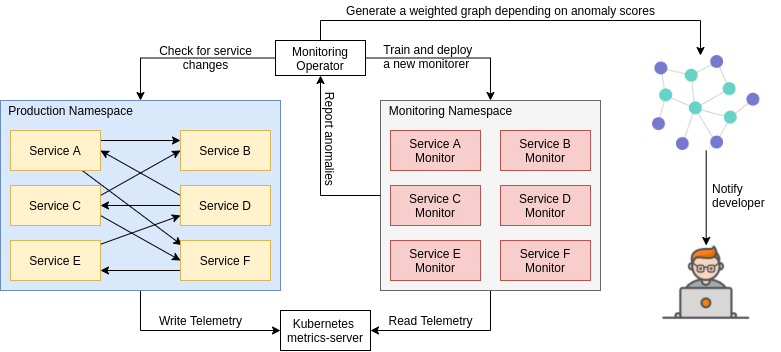
\includegraphics[width=16cm]{assets/High-level-system-diagram.png}
    \caption{Prototype feature diagram (self composed)}
    \label{fig:high-level-diagram}
\end{figure}
\section{Chapter Summary}

The above chapter described the participation of social, legal, ethical and professional issues in this project and how those were mitigated to comply with the BCS code of conduct.

\end{document}

